%==================================================
% Standard
%==================================================
\documentclass[11pt]{article} % Page setup
\usepackage[top=1in, bottom=1in, left=1in, right=1in]{geometry} % Margin setup
\usepackage[square,sort,comma,numbers]{natbib}  % Reference Formatting
\usepackage{fancyhdr} % Header setup
\usepackage[toc,page]{appendix}
\usepackage[hang,flushmargin]{footmisc}
\usepackage{textpos}

%==================================================
%Typesetting Packages
%==================================================

\usepackage{url} %Allows urls to be displayed properly
\usepackage{amsmath,amssymb} % Highly recommended as an adjunct to serious mathematical typesetting; amssymb provides extended symbol collection
\usepackage{amsthm} % proofs, lemmas, theorems
\usepackage{textcomp} % Package supports Text Companion fonts (baht, bullet, copyright, musicalnote, onequarter, section, and yen)
\usepackage{color} % Provides foreground (text, rules, etc.) and background color management
\usepackage{colordvi} % Allows for using named colors when typsetting output
\usepackage[usenames,dvipsnames,svgnames,table]{xcolor} % Extends the color package; several color tints, shades, tones, and mixes of arbitrary colors
\definecolor{arsenic}{rgb}{0.23, 0.27, 0.29}
\definecolor{color18}{rgb}{0.5,0.5,0.5} % Defines a color named "color18"
\usepackage{bm} % bold math
\usepackage{siunitx} % si units package 
\newcommand{\SIper}{\SI[per-mode=symbol]} % Special command for the SI unit package
\usepackage{enumerate} % Allows for the enumerate style to be changed 
%\usepackage{enumitem}
\usepackage{alphalph}
\usepackage{setspace}
\usepackage{blindtext}
\usepackage{soul}
\usepackage[tocindentauto]{tocstyle}
\usepackage{algorithm}
\usepackage{algpseudocode}
\usepackage{multirow}
\usepackage{mathtools}
\usepackage{afterpage}
\usepackage{float}
\usepackage{changepage}
\numberwithin{equation}{section}
%\usepackage{mathptmx}

% ==================================================
%Figure packages
% ==================================================
\usepackage{graphicx} % Include figure files
\usepackage{rotating} % Performs all rotations including complete figures and tables with their captions ON ONE PAGE
\usepackage{lscape} % Rotates the page contents but not the page number; can be applied across many pages
\usepackage[font=scriptsize,format=plain,labelfont=bf]{caption} % Caption customization (also for tables)
\usepackage{subcaption} % Provides support for subcaptions
\usepackage{float} % Improved interface for defining float objects (figures and tables)
\usepackage{wrapfig} % Allows figures or tables to have text wrapped around them
\setlength{\parskip}{5pt} %Space between paragraphs
\setlength{\parindent}{0pt} %Paragraph Indent size
\usepackage{fancybox}
\usepackage{mdframed}
\usepackage{makeidx}
\usepackage{tablefootnote}

% ==================================================
% Table packages
% ==================================================
\usepackage{longtable} % allow multipage tables
\usepackage{multicol}
\usepackage{multirow} % create tabular cells spanning multiple rows
\usepackage{dcolumn} % Align table columns on decimal point
\usepackage{threeparttable}
\usepackage{lipsum,booktabs}

% ==================================================
% Section Formatting 
% ==================================================
\usepackage{sectsty}
\allsectionsfont{\bfseries} %Sets ALL section font

%Title, author, date formats	
	\newcommand{\mytitle}[1]{\title{\bf{\textsf{#1}}}}
	\newcommand{\myauthor}[1]{\author{\textsf{#1}}}
	\newcommand{\mydate}[1]{\textsf{\date{#1}}}
	\newcommand{\mytoday}{\textsf{\today}}

%Section header formats	(Numbered)
	\newcommand{\mysection}[2]{\vspace{-5px}\section{#1}\label{#2}\vspace{-10px}}
	\newcommand{\myssection}[2]{\vspace{-5px}\subsection{#1}\label{#2}\vspace{-5px}}
	\newcommand{\mysssection}[2]{\vspace{-5px}\subsubsection{#1}\label{#2}\vspace{-5px}}

%Section header formats	(Unnumbered)	
	\newcommand{\mysectionN}[2]{\vspace{-5px}\section*{#1}\label{#2}\vspace{-10px}}
	\newcommand{\mysectionnonum}[2]{\vspace{-5px}\section*{#1}\label{#2}\vspace{-10px}}
	\newcommand{\myssectionN}[2]{\vspace{-5px}\subsection*{#1}\label{#2}\vspace{-5px}}
	\newcommand{\myssectionnonum}[2]{\vspace{-5px}\subsection*{#1}\label{#2}\vspace{-5px}}
	\newcommand{\mysssectionN}[2]{\vspace{-5px}\subsubsection*{#1}\label{#2}\vspace{-5px}}
	\newcommand{\mysssectionnonum}[2]{\vspace{-5px}\subsubsection*{#1}\label{#2}\vspace{-5px}}

%Paragraph header formats		
	\newcommand{\mypart}[2]{\part{#1}}
	\newcommand{\mypara}[2]{\paragraph{#1}}
	\newcommand{\myparaN}[2]{\paragraph*{#1}}
	\newcommand{\myparanonum}[2]{\paragraph*{#1}}


% ==================================================
% References, hyperrefs etc.
% ==================================================
\usepackage[colorlinks=true,linkcolor=Blue,citecolor=Red,urlcolor=Blue]{hyperref} % sets the color of hyperlinks
	\newcommand{\myref}[2]{\hyperref[#2]{#1~\ref{#2}}}
	\newcommand{\myrefexp}[3]{\hyperref[#3]{{#1}~{#2}}}
	\newcommand{\hilight}[1]{\colorbox{yellow}{#1}}
	\newcommand{\myfilename}[1]{\texttt{\textsf{#1}}}
	\newcommand{\mywebsite}[1]{\myfilename{\bf #1}}
	\newcommand{\commandline}[1]{\texttt{> #1}}
	\newcommand{\plusplus}[1]{#1{}\texttt{++}}

%Callout Box Creator	
	\newcommand{\callout}[3]
	{
	\begin{wrapfigure}{#1}{#2\textwidth}
	\vspace{-20pt}
	\centering
	\fbox{\parbox{#2\textwidth}{#3}}
	\vspace{-10pt}
	\end{wrapfigure}
	}

% ==================================================
% Track changes and commenting packages and commands
% ==================================================
\usepackage{todonotes}
	\newcommand{\sn}[1]{\todo[color=magenta!40,caption={}]{#1}}


	%Other colors available 
	%cyan
	%green
	%white
	%darkgray
	%brown
	%olive
	%pink
	%purple
	%violet


\usepackage{minted}
 


\newcommand{\bs}{\boldsymbol}
\renewcommand{\st}{\text{ s.t. }}
\newcommand{\eps}{\varepsilon}
\newcommand{\s}{\;}
\newcommand{\sif}{\text{ if }}
\newcommand{\pfrac}{\displaystyle \frac}
\newcommand{\Tau}{\mathcal{T}}
\newcommand{\Tref}{\mathcal{T}_{\text{ref}}}
\newcommand{\Qref}{\mathcal{Q}_{\text{ref}}}
\newcommand{\bb}[1]{\mathbb{#1}}

\newtheorem{theorem}{Theorem}[section]
\newtheorem{corollary}{Corollary}[theorem]
\newtheorem{lemma}{Lemma}[section]
\newtheorem{definition}{Definition}[section]
\newtheorem{proposition}{Proposition}[section]
\newtheorem{corollaryprop}{Corollary}[proposition]

\title{Sparse Spectral Methods on the Simplex}
\author{Sachin Natesh}
\date{\today}

\begin{document}
	\setcounter{secnumdepth}{5}
	\setcounter{tocdepth}{4}
\maketitle
\tableofcontents
\newpage
%	\begin{textblock*}{8cm}(15.5cm,-1cm)
%		\noindent {Sachin Natesh} 
%	\end{textblock*}

% ******************************************

\mysection{Jacobi ladders for sparse discrete operators in 1D}{}
We construct a sparse discrete differential operator for general, linear, two-point boundary value problems on $[-1,1]$. Our modal discretization will approximate the coefficients of the solution expanded in the Jacobi polynomial basis. The problem we will consider is
\begin{align}\label{eq:prob}
p(x)u''(x) + r(x)u'(x) + q(x)u(x) &= f(x),\s x \in (-1,1)\\
\alpha_1u(-1) + \alpha_2u'(1) &=\alpha,\label{eq:probbc0}\\ \beta_1u(-1)+\beta_2u'(1) &= \beta,\label{eq:probbc}
\end{align}
with $\alpha,\alpha_i,\beta,\beta_i\in \bb{R}.$
\myssection{Jacobi polynomials}{sec:1.1}
Consider the Jacobi polynomials $P_k^{(a,b)}(x)$ of order $k$ with parameters $a,b \in \bb{R}$ such that $a,b> -1$. These are orthogonal polynomials with respect to the weight function $w(x)=(1-x)^a(1+x)^b$ on the interval $[-1,1]$. While the polynomials can be explicity given in terms of the hypergeometric function, we list here only a few special cases, recurrence relations, and properties of relevance to our goal of constructing sparse discretized operators in 1D. 

Let scalars $q,r,s,t$ be defined in terms of the order and parameters $(k,a,b)$ by
\begin{equation}
\begin{split}
q &= k^2(k+a+b)(k^2+a+b-2),\\
r &= (k^2+a+b-1)(a^2-b^2),\\
s &= (k^2+a+b-2)(k^2+a+b-1)(k^2+a+b),\\
t &= 2(k+a-1)(k+b-1)(k^2+a+b).
\end{split}
\end{equation}
Then, we can completely specify $P_k^{(a,b)}$ for any $k$:
\begin{equation}\label{eq:jacdef}
\begin{split}
P_0^{(a,b)}(x) &= 1,\\
P_1^{(a,b)}(x) &= \frac{1}{2}\big((a+b+2)(x-1)+2(a+1)\big),\\
P_{k\geq 2}(x)^{(a,b)} &=\big((r+sx)P_{k-1}^{(a,b)}(x) - tP_{k-2}^{(a,b)}(x)\big)/q.
\end{split}
\end{equation}
The polynomials satisfy the following orthogonality relation
\begin{equation}\label{eq:ortho}
\int_{-1}^1 (1-x)^a(1+x)^bP_i^{(a,b)}(x)P_j^{(a,b)}(x)dx = \frac{2^{a+b+1}}{2j+a+b+1}\frac{\Gamma(j+a+1)\Gamma(j+b+1)}{\Gamma(j+a+b+1)j!}\delta_{ij},
\end{equation}
and for $i=j$, the right hand side of \eqref{eq:ortho} gives us the squared normalization factor for the polynomials. For the orthonormal polynomials expressed in the recurrence form of \eqref{eq:orthrec}, the coefficients are 
\begin{align}
a_{k>0} &= \frac{2}{a+b+2k+2}\Big(\frac{(a+k+1)(b+k+1)(k+1)(a+b+k+1)}{(a+b+2k+1)(a+b+2k+3)} \Big)^{1/2},\\
a_0 &= \frac{2}{a+b+2}\Big(\frac{(a+1)(b+1)}{a+b+3}\Big)^{1/2},\\
b_{k>0} &= -B_k/A_k,\quad  b_0 = \frac{\frac{1}{2}(b-a)}{\frac{1}{2}(a+b)+1},
\end{align}
where $A_k,B_k$ are given in \cite[Eq. 18.9.2]{DLMF}. We also note the following properties:
\begin{enumerate}[(i)]
	\item $P_k^{(a,b)}(-1) = (-1)^k {k+b\choose k}$
	\item $P_k^{(a,b)}(1) = {k+a \choose k}$
	\item $P_{-1}^{(a,b)}(x) = 0$ (convention we will adopt)
\end{enumerate}
\myssection{Ladder operators}{sec:1.2}
There exist so called ladder operators which relate $P_k^{(a,b)}$ to another Jacobi polynomial with either the order $k$ or parameters $a,b$ incremented or decremented \cite{jacladder}. Here, we will consider the first ladder operation $\mathcal{L}_1$, given by
\begin{equation}\label{eq:ladder}
\mathcal{L}_1 P_k^{(a,b)} = \frac{1}{2}(k+a+b+1)P_{k-1}^{(a+1,b+1)} = \frac{d}{dx}P_k^{(a,b)}.
\end{equation}
That is, $\mathcal{L}_1$ relates the $(k,a,b)$ polynomial to its derivative in terms of $(k-1,a+1,b+1)$ polynomial. Applying $\mathcal{L}_1$ to $P_k^{(a,b)}$ gives a similar relation for its second derivative;
\begin{align}\label{eq:ladder2}
\frac{d^2}{dx^2}P_k^{(a,b)} &= \frac{1}{4}(k+a+b+1)(k+a+b+2)P_{k-2}^{(a+2,b+2)}, \quad k \geq 2 \\
\frac{d^2}{dx^2}P_k^{(a,b)} &= 0, \quad k = 0,1 \label{eq:ladder2_1}
\end{align}
where now the order and parameters have been, respectively, decremented and incremented by 2.
\myssection{Promotion operators}{}
Consider an ODE with highest derivative order $l$, and suppose we represent the solution, RHS and coefficient functions by Jacobi polynomials with parameters $(a,b)$. We showed in the next section that these representations must be promoted to $(a+l,b+l)$ to match the coefficients of the highest derivative obtained by the ladder operation. In \myref{Section}{sec:numexp}, we numerically demonstrate that greater Jacobi parameters lead to instability for increasing polynomial order. However, one can derive by $L^2$-projection the promotion operators relating the Jacobi polynomial $P_k^{(a,b)}$ to $P_k^{(a+1,b+1)}$, as done in \cite{promote}. 

That is, if $\bs{f}^{a,b} = [f_0,\cdots,f_N]^T$ are the expansion coefficients of $f(x)$ in the basis given by rows of $\bs{P}^{(a,b)}(x) = [P_0^{(a,b)}(x),\cdots,P_N^{(a,b)}(x)]^T$, i.e. $$f(x) \approx [\bs{P}^{(a,b)}(x)]^T\bs{f}^{(a,b)} ,$$
then there exists a matrix $\mathcal{K}_{(a,b)}^{(a+1,b+1)}$ such that
\begin{equation}
	\bs{f}^{(a+1,b+1)} = \mathcal{K}_{(a,b)}^{(a+1,b+1)}\bs{f}^{(a,b)}.
\end{equation}
In particular, $\mathcal{K}_{(a,b)}^{(a+1,b+1)}$ is the upper triangular matrix
\begin{equation}
\mathcal{K}_{(a,b)}^{(a+1,b+1)}	= \begin{bmatrix}
		\lambda_1^{(a,b,0)} & \lambda_2^{(a,b,0)} & \lambda_3^{(a,b,0)} & &\\
		& \lambda_1^{(a,b,1)} & \lambda_2^{(a,b,1)} & \ddots &\\
		& & \ddots & \ddots & \lambda_3^{(a,b,N-2)}\\
		& & & \ddots & \lambda_2^{(a,b,N-1)} \\
		& & & & \lambda_1^{(a,b,N)}
	\end{bmatrix}
\end{equation}
with diagonal entries
\begin{equation}
	\begin{split}
		\lambda_1^{(a,b,i)} &= \frac{(a+b+i+1)(a+b+i+2)}{(a+b+2i+1)(a+b+2i+2)}\\
		\lambda_2^{(a,b,i)} &= \frac{(a-b)(a+b+i+2)}{(a+b+2i+2)(a+b+2i+4)}\\
		\lambda_3^{(a,b,i)} &= -\frac{(a+i+2)(b+i+2)}{(a+b+2i+4)(a+b+2i+5)}.
	\end{split}
\end{equation}
Hence, we can construct an upper triangular promotion operator of order $l$ through
\begin{equation}
	\mathcal{K}_{(a,b)}^{(a+l,b+l)}  = \mathcal{K}_{(a+l-1,b+l-1)}^{(a+l,b+l)}\cdots \mathcal{K}_{(a+1,b+1)}^{(a+2,b+2)}\cdot \mathcal{K}_{(a,b)}^{(a+1,b+1)},
\end{equation}
which will promote $\bs{f}^{(a,b)}$ to $\bs{f}^{(a+l,b+l)}$
\myssection{Modal multiplication operator}{}
Our model discretization of \eqref{eq:prob} will require us to represent multiplications involving ODE coefficient functions in the modal basis. For example, we need to construct an operator which will map the coefficients of $u$ to those of $q(x)u(x)$. 

\mysssection{Multiplication by $x$}{}
Recurrence relations of the form of \eqref{eq:ogrec} naturally provide a \underline{``multiplication by $x$''} operator, which, given coefficients of $f$, maps to the coefficients of the product $xf$. For $\bs{P}(x) \in \bb{R}^n$ we have
\begin{equation}
x\bs{P}(x) = \mathcal{J}_n\bs{P}(x) + a_{n-1}P_n(x)\bs{e}_n,
\end{equation}
where $\mathcal{J}_n$ is the tridiagonal Jacobi matrix encoding the recurrence (see \eqref{eq:jacobimat} for the orthonormal case) given by
\begin{equation}\label{eq:jacobimatOG}
	\mathcal{J}_n = \begin{bmatrix}
		b_0 & a_0 & & &\\
		c_1 & b_1 & a_1 & & \\
		& c_2 & \ddots & \ddots & \\
		& & \ddots & b_{n-2} & a_{n-2}\\
		& & & c_{n-2} & b_{n-1}
	\end{bmatrix},
\end{equation}
and $\bs{e}_n$ is the $n^{th}$ standard basis vector. Consider the Jacobi expansion of $f(x) \approx \bs{f}^T \bs{P}(x)$, and the product $xf(x)$:
\begin{align}\label{eq:orthprojmult}
xf(x) &\approx x\bs{P}(x)^T\bs{f} = \big( \bs{P}(x)^T \mathcal{J}_n^T + \begin{bmatrix} 0 & \cdots & 0 & a_{n-1}P_n(x)\end{bmatrix}\big)\bs{f}
\end{align}

If we evaluate the above expression for $\bs{x}$ a discrete $n$ point grid from $-1$ to $1$ (row vector), we see that $[\bs{P}(\bs{x})]^T$ is the Vandermonde matrix, and the component-wise product is
\begin{equation}\label{eq:mbyx}
[\bs{x}\odot f(\bs{x})]^T \approx \bs{P}(\bs{x})^T\big(\mathcal{J}_x \bs{f}\big), \text{ where } \mathcal{J}_x = \Big(\mathcal{J}_n^T +  \bs{P}(\bs{x})^{-T}\begin{bmatrix} \bf{0}_{n\times n-1} & a_{n-1}P_n(\bs{x}^T)\end{bmatrix}\Big)
\end{equation}
Markedly, $\mathcal{J}_n^T$ is the \color{red} orthogonal projection operator composed with the multiplication operator. It takes the modes of $f(x)$ and computes the modes of the projection of $xf(x)$ in the span of $\bs{P}(x)$ \color{black}. $\mathcal{J}_x$ is our modal multiplication-by-$x$ operator, and $\mathcal{J}_x^l$ represents multiplication by $\bs{x}^{\circ l}$ (Hadamard power), as in 
\begin{equation}
[\bs{x}^{\circ l} \odot f(\bs{x})]^T \approx \bs{P}(\bs{x})^T\big(\mathcal{J}_x^l \bs{f})
\end{equation}

\mysssection{Multiplication by $g(x)$}{}
We can use the multiplication operators to construct a general operator which can map the coefficients of $f$ to those of the product $fg$ for any function $g$. To see this, suppose $f$ and $g$ are represented in Jacobi bases of possibly different degrees $n-1,m-1$. Then, by the equivalent representation of $g$ in the monomial basis $\tilde{\bs{P}}(x) = [1,x,\cdots,x^{m-1}]^T$ with coefficients $\tilde{\bs{g}}$,
\begin{align*}
[f(\bs{x})\odot g(\bs{x})]^T &\approx f(\bs{x})^T \odot \big(\bs{P}(\bs{x})^T \bs{g}\big) = f(\bs{x})^T \odot \big(\tilde{\bs{P}}(\bs{x})^T \tilde{\bs{g}}\big) \\&=  \Big(\sum_{j=0}^{m-1} \tilde{g}_j [\bs{x}^{\circ l} \odot f(\bs{x})]^T\Big) = \bs{P}(\bs{x})^T\Big(\sum_{j=0}^{m-1}\tilde{g}_j\mathcal{J}_x^l\Big)\bs{f}\\
&\approx \bs{P}(\bs{x})^T \Big(g(\mathcal{J}_x)\bs{f}\Big),
\end{align*}
where $g(\mathcal{J}_x)$ is approximated in terms of the Jacobi polynomial expansion given matrix input. Thus, given an $n\times n$ multiplication-by-$x$ operator $\mathcal{J}_x$ for approximating the $n$ coefficients of $xf(x)$, the \underline{multiplication-by-$g$} operator for $f$ is simply
\begin{equation}
	\mathcal{M}_g = g(\mathcal{J}_x),
\end{equation}  
and allows us to approximate the $n$ expansion coefficients of $f(x)g(x)$ by $M_g \bs{f}$.

We can generalize \underline{Clenshaw's algorithm} \cite{Clenshaw} for operator valued input to evaluate $g(\mathcal{J}_x)$ given the Jacobi expansion coefficients of $g$. The scalar-valued Clenshaw algorithm is derived by first recasting the recurrence \eqref{eq:ogrec} as the set of equations $\{P_0 = 1,\s a_n P_{n+1} + (b_n-x)P_n + c_nP_{n-1}= 0\}$. Then, as a matrix equation with $\bs{e}_1 \in \bb{R}^n$ the first standard basis vector, we have
\begin{equation}
\mathcal{C}\bs{P}(x) = \bs{e}_1,\quad 
\mathcal{C} = \begin{bmatrix}
	1 & & & &\\
	b_0-x & a_0 & & &\\
	c_1 & b_1-x & a_1 & & \\
	& \ddots & \ddots & \ddots & \\
	& & c_{n-3} & b_{n-2}-x & a_{n-2}
\end{bmatrix},	
\end{equation}
so that 
\begin{equation}
	g(x) = \bs{P}(x)^T \bs{g} = \bs{e}_1^T(\mathcal{C}^{-T}\bs{g})
\end{equation}
The operator valued algorithm follows analogously. Let $I$ be the $n\times n$ identity matrix and $\bs{e}_1 \in \bb{R}^m$ the first standard basis vector (of length $m$). We know that $\bs{P}(\mathcal{J}_x)$ is an $m$-length block column vector with $n\times n$ blocks. Then,
\begin{equation}
\mathcal{C}\bs{P}(\mathcal{J}_x) = (\bs{e}_1 \otimes I),\quad \mathcal{C} = \begin{bmatrix}
	I & & & &\\
	b_0I-\mathcal{J}_x & a_0I & & &\\
	c_1I & b_1I-\mathcal{J}_x & a_1I & & \\
	& \ddots & \ddots & \ddots & & \\
	& & c_{n-3}I & b_{n-2}I-\mathcal{J}_x & a_{n-2}I
\end{bmatrix},
\end{equation}
so that
\begin{equation}
	\mathcal{M}_g = g(\mathcal{J}_x) = \bs{P}(\mathcal{J}_x)^T(\bs{g}\otimes I) = (\bs{g} \otimes I)^T\big[\mathcal{C}^{-1}(\bs{e}_1 \otimes I)\big].
\end{equation}
Here, $\mathcal{C} \in \bb{R}^{mn\times mn}$ and contains $m$ blocks of size $n\times n$ on the main diagonal. We have actually revealed a \underline{multiplication-by-$\star$} operator, i.e.
\begin{equation}
\mathcal{M}_{\star} = \mathcal{C}^{-1}(\bs{e}_1\otimes I), \quad \mathcal{M}_g = (\bs{g} \otimes I)^T \mathcal{M}_\star,
\end{equation}
which can be precomputed given the expansion of $f$, and reused to construct $\mathcal{M}_g$ for an arbitrary function $g$. 
\myssection{Sparsity patterns of the multiplication operator}{}
For variable coefficient problems, it is desirable that the coefficients can represented by a polynomial of degree $M \leq N$, where $N$ is the representation order for the solution. If $M=N$, then $\mathcal{M}_g$ is completely filled in. As $M$ decreases, $M$ develops a banded structure. Hence, the max polynomial degree for representing the coefficient functions should be carefully selected. Moreover, if $M > N$, the multiplication operators will not resolve the products well. In \myref{Figure}{fig1}, we show the sparsity pattern of $M_g$ for $g(x) = \{x^2,x^3,x^4\}$ given $f(x) = e^{x\cos(x)}$. We need $M+1$ points to represent a polynomial of degree $M$, and each extra degree adds 2 to the bandwidth of the block diagonal part of $\mathcal{M}_g$. 
\begin{figure}[H]
	\centering
	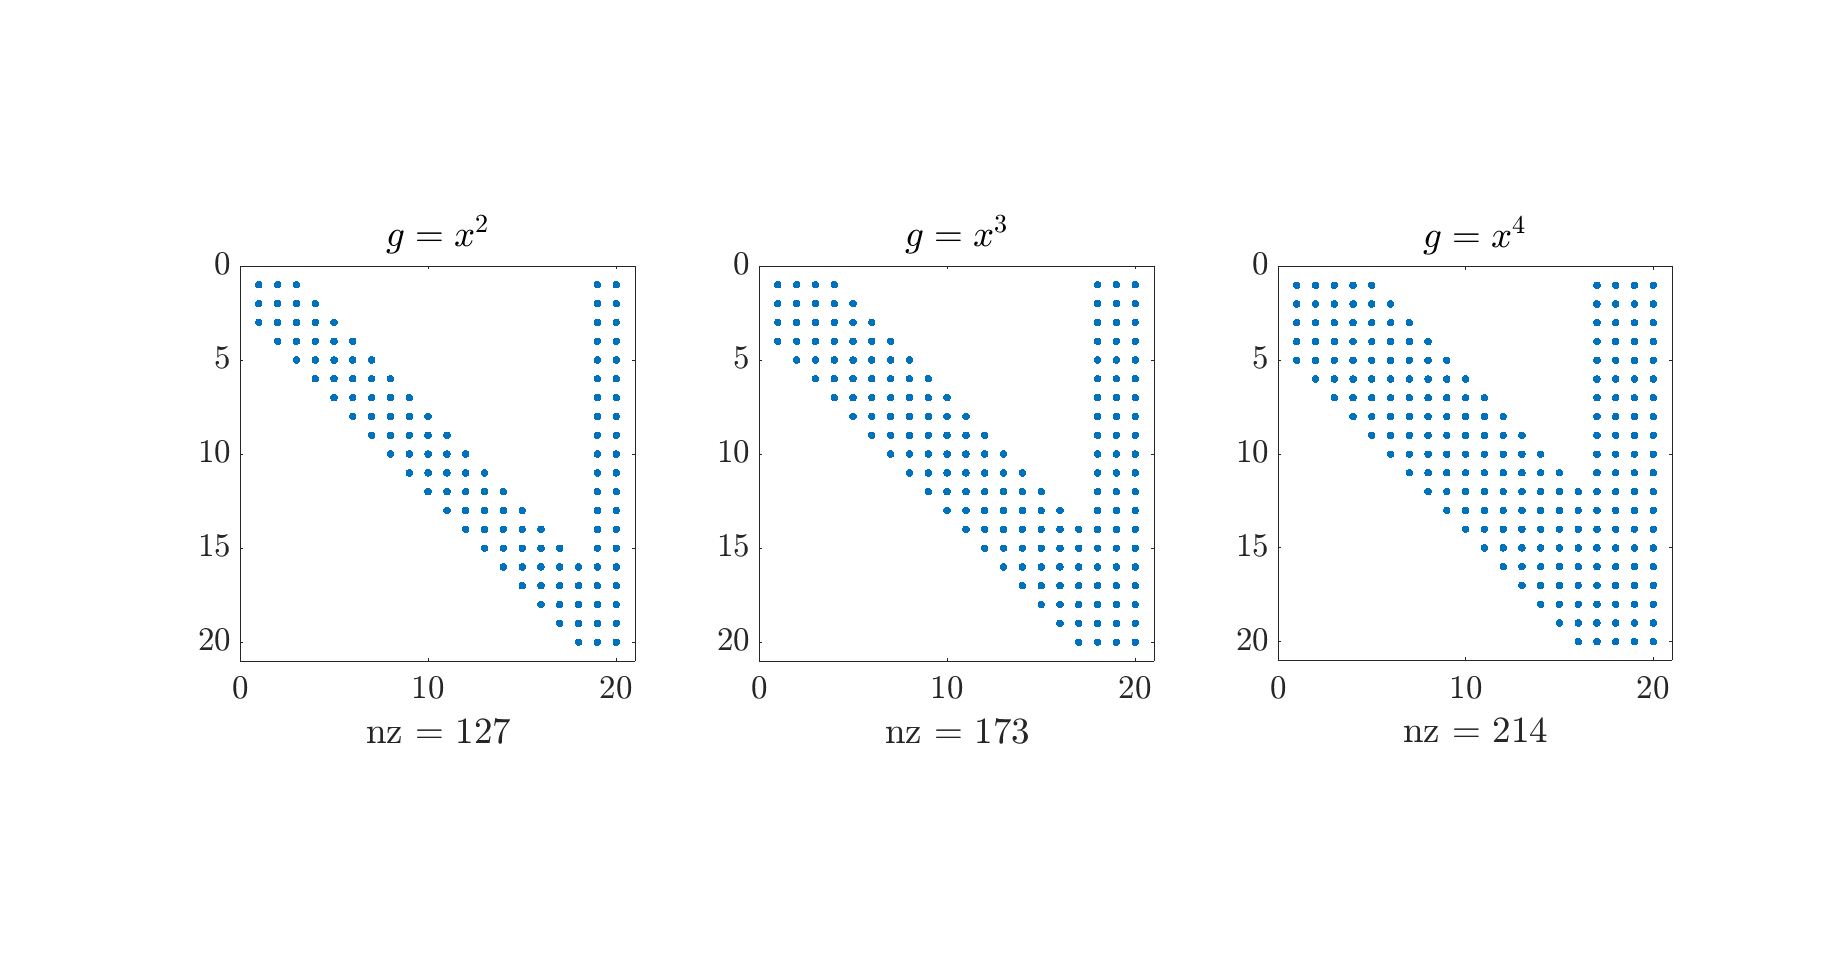
\includegraphics[width=\linewidth,trim=4cm 4cm 4cm 4cm,clip]{figures/Mg_sparse}
	\caption{Sparsity pattern for $\mathcal{M}_g$ given $f(x) = e^{x\cos(x)}$. We used $N=20$ points to represent $f$ (degree $N-1$).}\label{fig1}
\end{figure}

\myssection{Constructing the sparse differential operator}{}
Equipped with our ladder, promotion and multiplication operators, we can now construct a sparse differential operator for \eqref{eq:prob}-\eqref{eq:probbc}. First, we consider an $N^{\text{th}}$  degree polynomial approximation for $u$, and $M_q,M_r,M_p$ degree approximations for the coefficient functions $p,r,q$. For example,
\begin{equation}\label{eq:ujac1}
u(x) \approx \sum_{k=0}^Na_kP_k^{(a,b)}(x).
\end{equation}
Inserting \eqref{eq:ujac1} into \eqref{eq:prob} and applying \eqref{eq:ladder}-\eqref{eq:ladder2_1}, we find
\begin{equation}\label{eq:u''jac}
\begin{split}
u''(x) &\approx \sum_{k=2}^N \Big(\frac{a_k}{4}(k+a+b+1)(k+a+b+2)\Big)P_{k-2}^{(a+2,b+2)}(x),\\
u'(x) &\approx \sum_{k=1}^N \frac{a_k}{2}(k+a+b+1)P_{k-1}^{(a+1,b+1)}(x)
\end{split}
\end{equation}
According to \eqref{eq:u''jac}, there exists linear mappings, which we denote $\mathcal{D}^2 : \bb{R}^{N+1}\to \bb{R}^{N+1}$, and $\mathcal{D}$ that relates the Jacobi coefficients of $u$ to those of $u''$, and $u'$ respectively. Explicitly, for $i,j = 0,1,\cdots N$, the entries of $\mathcal{D}^2$ are given by
\begin{equation}\label{eq:D2}
\mathcal{D}^2_{ij} = 
\begin{cases} \frac{1}{4}(a+b+j+1)(a+b+j+2)&,\quad j = i+2\\
0&, \quad j \neq i + 2,
\end{cases}
\end{equation}
and those of $\mathcal{D}$ are given by
\begin{equation}
\mathcal{D}_{ij} = 
\begin{cases} \frac{1}{2}(a+b+j+1)&,\quad j = i+1\\
	0&, \quad j \neq i + 1,
\end{cases}	
\end{equation}
We see that $\mathcal{D}^2 \bs{a}$ gives the Jacobi coefficients of $u''$ in the basis of $\bs{P}^{(a+2,b+2)}$. That is,
\begin{equation}
u''(x) \approx (\mathcal{D}^2 \bs{a})^T \bs{P}^{(a+2,b+2)}(x).
\end{equation}
Assuming the coefficients of $p,r,q$ are appropriately promoted, we can use the multiplication operator to explicitly write the discrete modal operator:
\begin{equation}
\begin{split}
\mathcal{L} &= 
\mathcal{M}_p\mathcal{D}^2 + \mathcal{M}_r\mathcal{K}_{(a+1,b+1)}^{(a+2,b+2)} \mathcal{D} + \mathcal{M}_q\mathcal{K}_{(a,b)}^{(a+2,b+2)},\\
\mathcal{L}\bs{a} &= \mathcal{K}_{(a,b)}^{(a+2,b+2)}\bs{f}.
\end{split}
\end{equation}

As is, $\mathcal{L}$ is not invertible. However, we can add the independent boundary conditions \eqref{eq:probbc0}-\eqref{eq:probbc} to eliminate the rank deficiency. By properties (ii) and (iii) in \myref{Section}{sec:1.1}, and using the first ladder operator, we have that 
\begin{equation}
\begin{split}
u(-1) &\approx \sum_{k=0}^N (-1)^k {k+b \choose k} a_k,\quad u(1) \approx \sum_{k=0}^N {k+a \choose k}a_k \\
u'(-1) &\approx \sum_{k=1}^N \frac{k+a+b+1}{2}(-1)^k{k+b+1\choose k} a_k,\quad u(1) \approx \sum_{k=1}^N \frac{k+a+b+1}{2}{k+a+1\choose k}a_k
\end{split}
\end{equation}
Hence, we can define a modified operator $\hat{\mathcal{L}}$ with same entries as $\mathcal{L}$, except
\begin{equation}\label{eq:D2hat}
\hat{\mathcal{L}}_{ij} = 
\begin{cases} \mathcal{L}_{ij}&,\quad i \leq N-2\\
\alpha_1(-1)^j{j+b\choose j}&,\quad i = N-1,\s j = 0\\
\alpha_1(-1)^j{j+b\choose j} + \alpha_2 \frac{j+a+b+1}{2}(-1)^j{j+b+1\choose j}&,\quad i = N-1,\s j\neq 0\\
\beta_1{j+a\choose j}&,\quad i=N,\s j = 0\\
\beta_1{j+a\choose j} + \beta_2 \frac{j+a+b+1}{2}{j+a+1\choose j}&,\quad i = N,\s j \neq 0
\end{cases}
\end{equation}
Now, if we expand $f(x) \approx \sum_{k=0}^N c_k P_k^{(a+2,b+2)}(x)$ (obtained by the promotion of $\bs{f}$), then we can approximate a solution to \eqref{eq:prob}-\eqref{eq:probbc} by solving
\begin{equation}\label{eq:discrete}
	\hat{\mathcal{L}}\bs{a} = \begin{pmatrix} \bs{\tilde{c}}\\\alpha\\\beta\end{pmatrix},
\end{equation}  
where $\bs{\tilde{c}} = (c_0,c_1,\cdots c_{N-2})^T$. \color{purple} Note, we have to expand $f$ in the basis of $\bs{P}^{(a+2,b+2)}$ in order to solve the modal system, while $\bs{a}$ are the coefficients of $u$ in the basis of $\bs{P}^{(a,b)}$. \color{black}  More generally, we can construct the operator $\mathcal{D}^l$ such that $\mathcal{D}^l\bs{a}$ gives the Jacobi coefficients of $\partial^l u$ in the basis of $\bs{P}^{(a+l,b+l)}$ by
\begin{equation}\label{eq:Dl}
\mathcal{D}^l_{ij} = 
\begin{cases}
\frac{1}{2^l}\prod_{k=1}^l(a+b+j+k)&,\quad j=i+l\\
0&,\quad j \neq i + l,
\end{cases}
\end{equation}
and $l$ boundary conditions must be added in a manner similar to \eqref{eq:D2hat} in order to eliminate the rank deficiency.

\myssection{Evaluating the Jacobi polynomial expansion coefficients}{}
If nodal exactness in the approximation for $f$ is not a concern, we will use a best least squares approximation in the weighted $L_2$ sense to compute the expansion coefficients. If nodal exactness is desired, we can directly invert the Jacobi Vandermonde matrix. Similarly, if $f$ is already a high order, accurate polynomial interpolant in a different basis, direct inversion gives an identical interpolant in the Jacobi basis, owed to the uniqueness of polynomial interpolation.
\mysssection{Weighted $L_2$ approximation}{}
Consider the polynomial expansion in the weighted $L_2$ sense of $f \in \Pi_N([-1,1])$ in the span of $\{P_j^{(a,b)}\}_{j=0}^N$;
\begin{equation}\label{eq:ujac}
f(x) = \sum_{j=0}^N c_jP_j^{(a,b)}(x),\quad c_j = \frac{1}{\sqrt{h_j}}\int_{-1}^1 f(x)p_j^{(a,b)}(x)w(x)dx,
\end{equation}
where $w(x)$ is the Jacobi weight function, $p_j^{(a,b)}$ are the normalized polynomials, and $h_j$ is the structure factor (as in \eqref{eq:ortho}) for $P_j^{(a,b)}$. This generalized Fourier series follows from the orthogonality of the Jacobi polynomials, and equality in the first term becomes $\approx$ if $f$ is not polynomial.

We can compute the coefficients $c_j$ using the Jacobi Vandermonde matrix.
%Suppose that we have an $2N+1$ point Clenshaw-Curtis-Jacobi quadrature rule on $[-1,1]$, capable of exactly integrating polynomials up to degree $2N$. Then, for any $f \in \bb{P}_N([-1,1])$ with best weighted $L_2$ expansion $f(x) \approx \sum_{j=0}^N c_jP_j^{(a,b)}(x)$, . 
To see this, suppose that we have an $M+1$ point quadrature rule on $[-1,1]$, capable of exactly integrating polynomials up to degree $2N$. For example, a Clenshaw-Curtis-Jacobi (CCJ) rule will require $M\geq 2N$, while a Gauss-Jacobi (GJ) rule requires $M\geq N$. Let $\{x_k\}_{k=0}^{M}$ with $-1\leq x_0<x_k<x_{M}\leq1$ be the quadrature nodes, $\bs{w}=(w_0,w_1,\cdots w_{M})^T$ the weights, and $\bs{f} = (f(x_0),f(x_1),\cdots f(x_{M}))^T$ the function values at the quadrature nodes.  

Using the recurrence relation in \eqref{eq:jacdef}, we can construct the $(M+1)\times(N+1)$ Vandermonde matrix $V$ with entries $V_{kj} = P_{j}^{(a,b)}(x_k)$. We also incorporate the structure factors from \eqref{eq:ortho} into a vector $\bs{h}$. Noting that $\text{deg}(fP_j^{(a,b)}) \leq 2N$,
\begin{align}\label{eq:jaccoeff}
c_j &= \frac{1}{\sqrt{h_j}}\int_{-1}^1 \frac{P_j^{(a,b)}(x)}{\sqrt{h_j}}f(x)w(x)dx = \frac{1}{h_j}\sum_{k=0}^{M}\big(P_j^{(a,b)}(x_k)f(x_k)\big)w_k \nonumber\\
\Rightarrow \bs{c} &= \Big(V^{T}\big(\bs{f} \odot \bs{w}\big)\Big)\oslash\bs{h},
\end{align}
where $\odot,\oslash$ are component-wise multiplication and division, respectively. If $\text{deg}(f) > N+1$, or if $f$ is not a polynomial, then the equality in \eqref{eq:jaccoeff} changes to $\approx$. \color{red} In \texttt{Chebfun}, it seems that they take this approach for converting between Chebyshev and Jacobi coefficients. However, this does not preserve the nodal exactness of the Chebyshev interpolant (easy to check). Moreover, we show in the next section that Clenshaw-Curtis type rules are unstable for larger $N$ and $a,b$. \color{black}
%
%If $f(x) = \sum_{j=0}^N b_jT_j(x)$ is a polynomial interpolant to another function $g(x)$ at the points $\{x_j\}$ in a different polynomial basis $\{T_j\}$, then $f(x) = \sum_{j=0}^N c_j P_j^{(a,b)}(x)$. Due to the uniqueness of polynomial interpolation, 


\mysssection{Direct inversion of the Vandermonde matrix}{}
The coefficients for the interpolant in the Jacobi polynomial basis are given by
\begin{equation}
\bs{c} = V^{-1}\bs{f},
\end{equation}
where $V$ is $(N+1) \times (N+1)$, and need not include any normalization factors.
\myssection{Numerical experiments}{sec:numexp}
Here, we provide convergence results for both Vandermonde inversion and weighted $L_2$ projection in approximating solutions to \eqref{eq:prob}-\eqref{eq:probbc} with $f(x)$ taken from $\big\{x,x^2,x^3,e^x\sin(x),\arctan(x)\big\}$. The solution nodes are the Chebyshev points $x_j = -\cos(j\pi/N)$ for $j=0,1,\cdots N$. In \myref{Figure}{fig:sols}, we show approximate solutions for each right-hand side $f(x)$.
\begin{figure}[H]
	\centering
	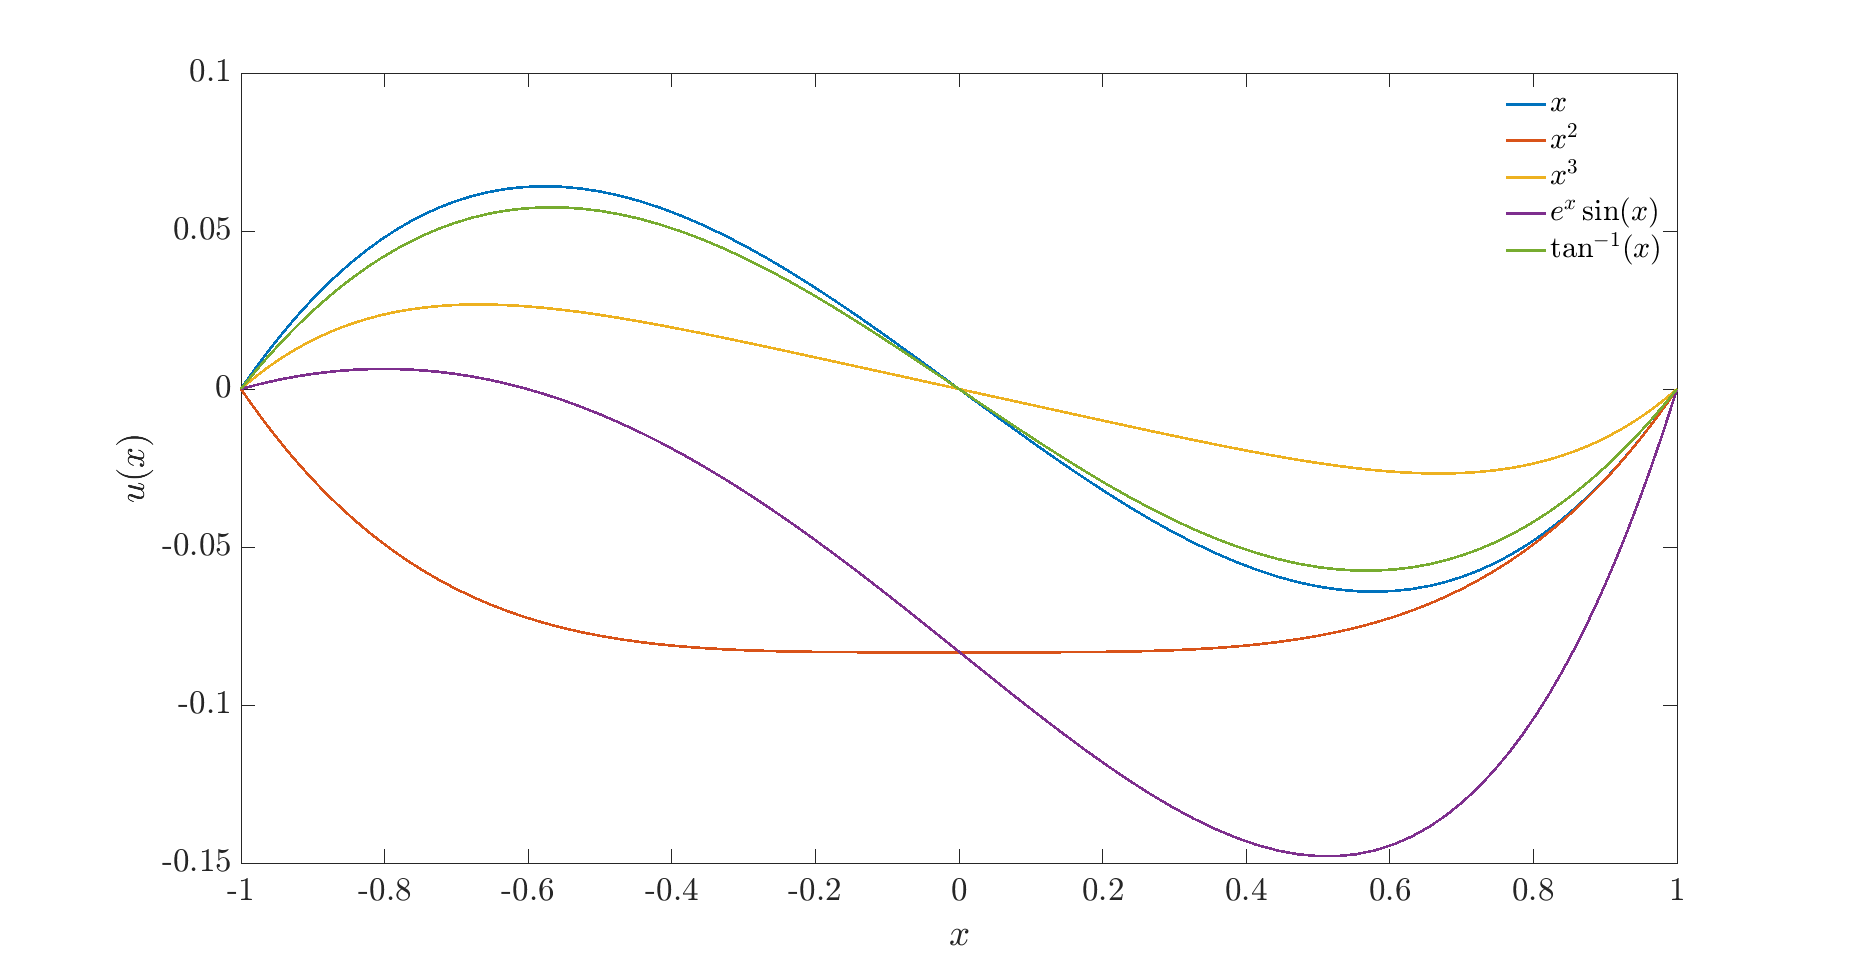
\includegraphics[width=0.64\linewidth]{./figures/sols}
	\caption{Solutions to \eqref{eq:prob}-\eqref{eq:probbc} for several right-hand sides.}\label{fig:sols}
\end{figure}

The error we report in \myref{Figure}{fig:errs} is the approximate interpolation error in the weighted $L_2$ norm. Given the solution coefficients $\bs{a}$, we compute
\begin{equation}
E^2(u) = \Big|\Big|u(x) - \sum_{j=0}^N a_jP_j^{(a,b)}(x)\Big|\Big|^2_{L_2^w([-1,1])}\approx \sum_{k=0}^M\Big(u(x_k)-\sum_{j=0}^N a_kP_j^{(a,b)}(x_k)\Big)^2w_k,
\end{equation}
where $\{x_k,w_k\}_{k=0}^M$ is an $M+1$ point quadrature rule ($M\gg N$). In words, we interpolate the approximate solution onto a fine $M+1$ point grid, and use the associated Gauss-Jacobi quadrature weights to approximate interpolation error. For these tests, we take $M=50$, and Jacobi parameters $(a,b) = (3,4)$. 
\begin{figure}[H]
	\centering
	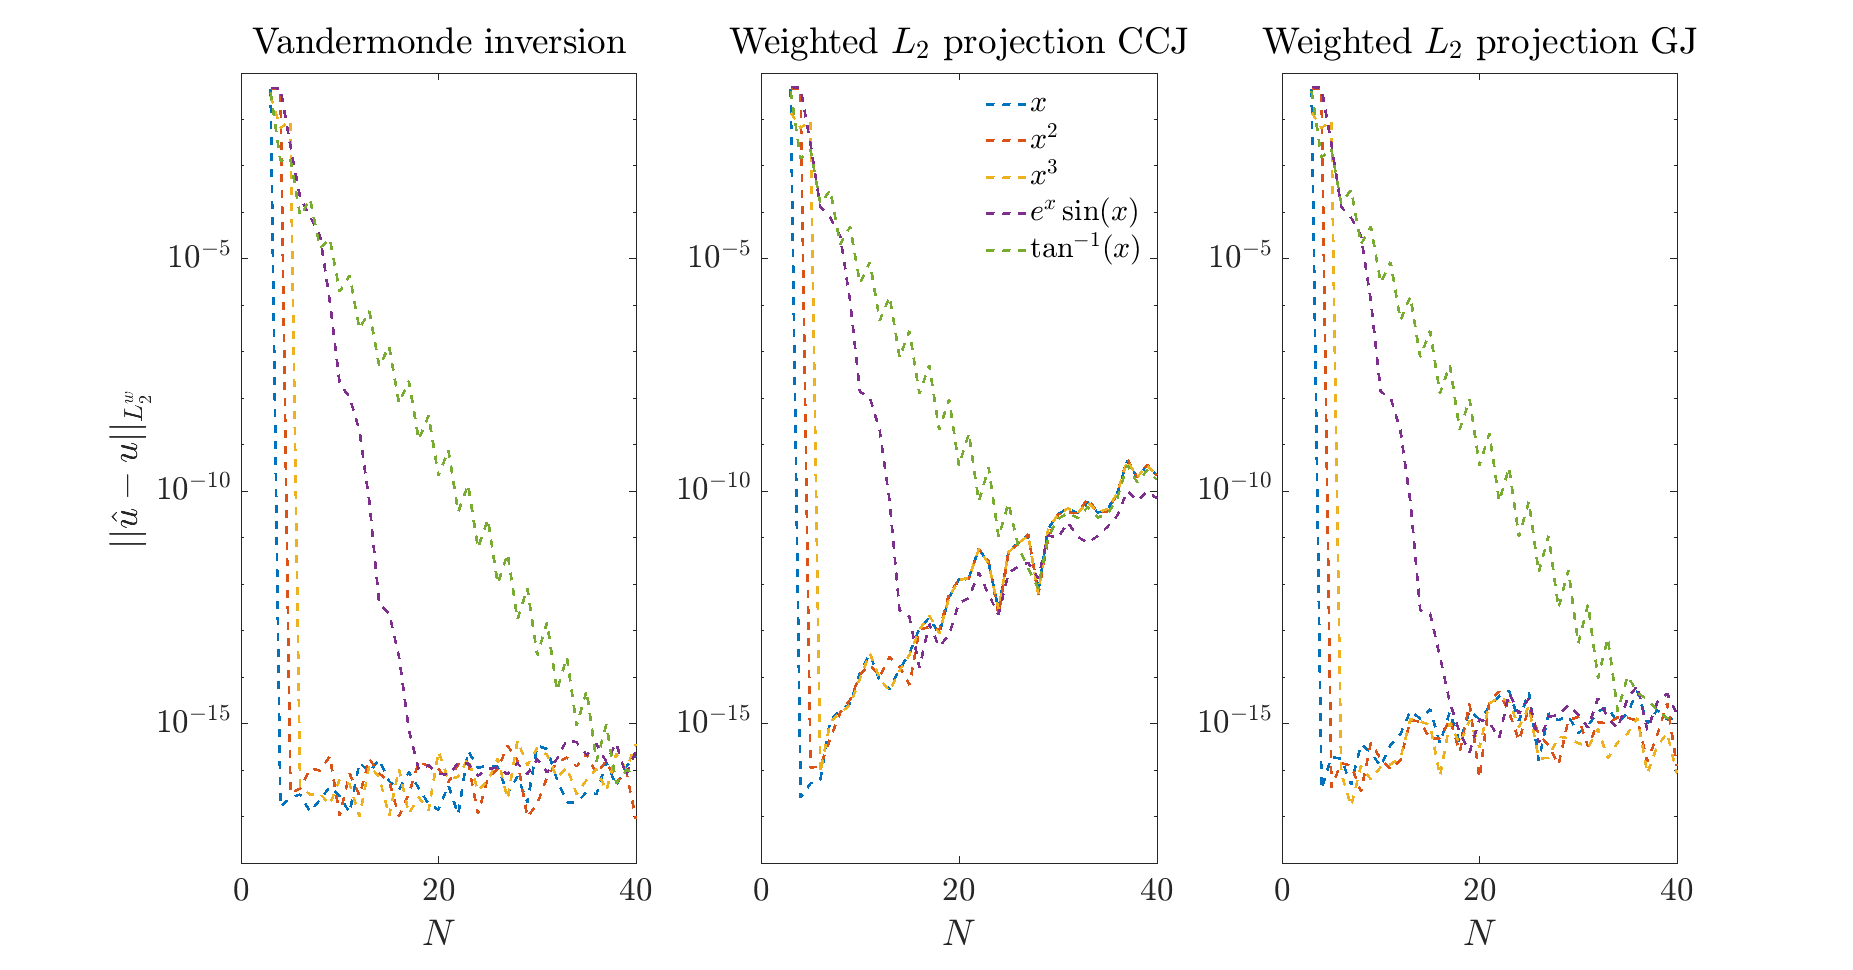
\includegraphics[width=1\linewidth]{./figures/errs}
	\caption{Weighted $L_2$ errors in approximate solutions to \eqref{eq:prob}-\eqref{eq:probbc} for several right-hand sides.}\label{fig:errs}
\end{figure}

We see that a polynomial right-hand side of degree $k$ requires $k+3$ points to approximate the solution to machine precision. Spectral convergence is observed for all $f$ considered. Moreover, Vandermonde inversion does not loose correct digits as $N\to \infty$, while the $L_2$ projection with CCJ quadrature is not as stable. On the other hand, GJ quadrature behaves more stably, like Vandermonde inversion. 

The instability is related to the Jacobi parameters $(a,b)$. For the problem of finding the best weighted $L_2$ coefficients (using the Clenshaw-Curtis type method in \eqref{eq:jaccoeff}) of a function $f$, larger values of $(a,b)$ lead to loss in digits for fixed $N$ large enough. This is illustrated in \myref{Figure}{fig:aberrs}, where with $N=20$, we compute the weighted $L_2$ error in the projection of $f(x)=e^x\sin(x)$ onto $\bs{P}^{(a,b)}$ for a range of $(a,b)$. Notice, for $a+b \in (-2,2)$, a regime which includes the Chebyshev and Legendre polynomials, the error decreases and is well controlled within $10^{-10}$ as $a$ and $b$ are incremented. On the other hand, the $a=b$ regime, corresponding to the ultraspherical (i.e. Gegenbauer) polynomials, and as well the $a,b>1$ regime, display an increase in error as $a$ and $b$ are incremented. For comparison, the right panel shows the same test with Gauss-Jacobi quadrature.

\begin{figure}[H]
	\centering
	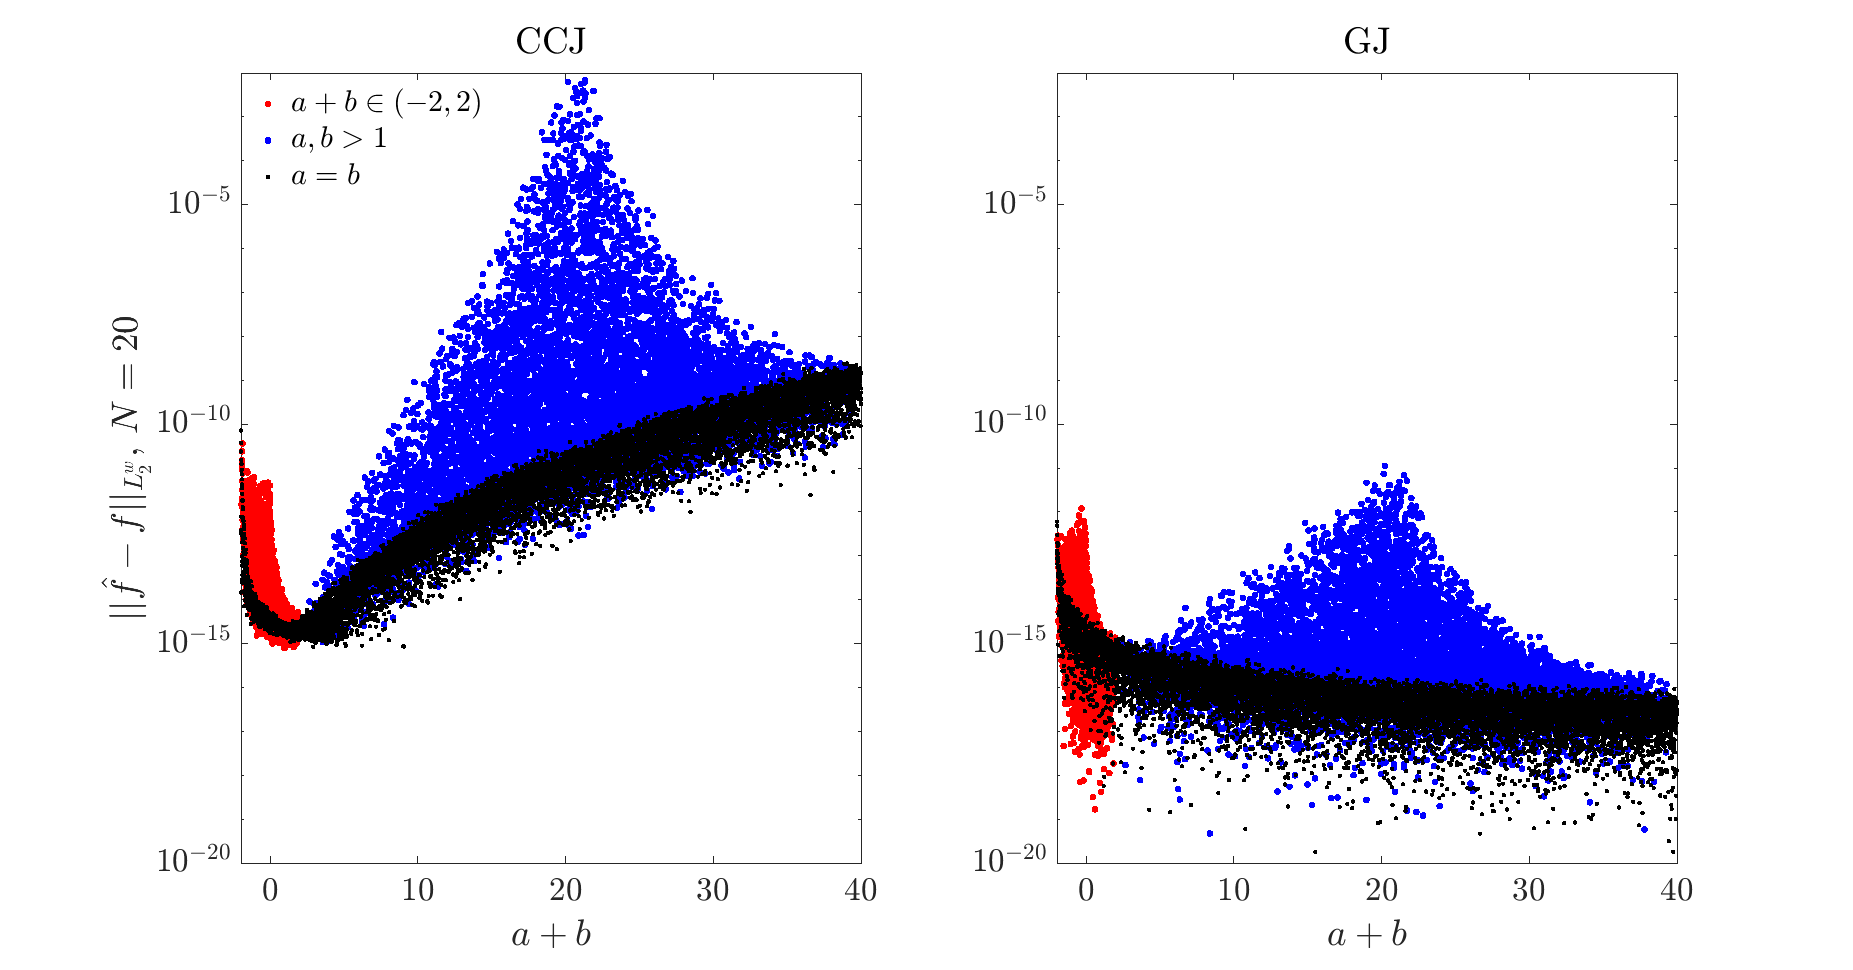
\includegraphics[width=1\linewidth]{./figures/aberr}
	\caption{Weighted $L_2$ errors in the projection of $f(x) = e^x\sin(x)$ onto $\bs{P}^{(a,b)}$ for various regimes in $(a,b)$ and $N=20$. CCJ is the Clenshaw-Curtis-Jacobi quadrature method, while GJ is Gauss-Jacobi.}\label{fig:aberrs}
\end{figure}

Hence, care must be taken when selecting the $(a,b)$ parameters to represent the solution of the differential equation, if the RHS $f$ is expressed via $L_2$ projection. Given that an order $k$ derivative will increment the parameters by $k$, the handling of high order equations is limited - unless a more stable quadrature is chosen to evaluate the integral in \eqref{eq:jaccoeff}.
%\begin{equation}\label{eq:D2}
%D^2 = \begin{pmatrix}
%0 & 0 & (a+b+3)(a+b+4) & 0 & 0 &\cdots & 0 \\
%0 & 0 & 0 & (a+b+4)(a+b+5) & 0 & \cdots & 0\\
%\vdots & \vdots &\vdots & &\ddots  & &\vdots \\
%0 & 0 & 0 & \cdots &  &  &(N+a+b+1)(N+a+b+2) \\
%
%\end{pmatrix}
%\end{equation}
\newpage
\mysection{Jacobi Ladders for Sparse Discrete Operators on the Triangle}{}
Here, we construct sparse differential operators for BVPs on the triangle $$\Tref^2 := \{(x,y)\s|\s 0\leq x,y,x+y\leq 1\}$$ using the classical orthogonal polynomials on this domain, due to Koornwinder. For starters, we want to solve Poisson's equation with Dirichlet data:
\begin{equation}\label{eq:laptri}
	\begin{split}
	\Delta u(x,y) &= f(x,y),\quad (x,y) \in \Tref^2\\
	u(x,y) &= g(x,y),\quad (x,y) \in \partial\Tref^2.
	\end{split}
\end{equation}
\myssection{Koornwinder polynomials}{sec:koornpoly}
To simplify notation in this section, $P_k^n$ denotes the $k^{\text{th}}$ Koornwinder polynomial of degree $n$ with parameters $(a,b,c)$. When the parameters must be specified, we will refer to the same polynomial by $P_{k,n}^{(a,b,c)}$. The weight function is
\begin{equation}\label{eq:koornweight}
	\begin{split}
	W(x,y) &= x^{a-\frac{1}{2}}y^{b-\frac{1}{2}}(1-x-y)^{c-\frac{1}{2}},\\
	w_{a,b,c} &= \Big(\int_{\Tref^2}W(x,y)dxdy\Big)^{-1}=\frac{\Gamma(|\kappa| + \frac{3}{2})}{\Gamma(a+\frac{1}{2})\Gamma(b+\frac{1}{2})\Gamma(c+\frac{1}{2})}
	\end{split}
\end{equation}
with $a,b,c > -1/2$ the Jacobi parameters, and $|\kappa| = a+b+c$. The orthonormal polynomials are given in terms of the 1D Jacobi polynomials by
\begin{equation}\label{eq:koornwinder}
\begin{split}
	P_k^n(x,y) &= (h_{k,n})^{-1}P_{n-k}^{2k+b+c,a-1/2}(2x-1)(1-x)^kP_k^{c-1/2,b-1/2}\Big(\frac{2y}{1-x}-1\Big),\\
	(h_{k,n})^2 &= \frac{w_{a,b,c}}{(2n+|\kappa|+\frac{1}{2})(2k+b+c)} \\
	          &\times \frac{\Gamma(n+k+b+c+1)\Gamma(n-k+a+\frac{1}{2})\Gamma(k+b+\frac{1}{2})\Gamma(k+c+\frac{1}{2})}{(n-k)!k!\Gamma(n+k+|\kappa|+\frac{1}{2})\Gamma(k+b+c)},
\end{split}
\end{equation}
and they satisfy a mutual orthonormality condition under the weighted inner product:
\begin{equation}\label{eq:koornorth}
	\langle P_j^m,P_k^n\rangle = \delta_{jk}\delta_{mn}. 
\end{equation}
That is to say, a given polynomial is not only orthonormal to those with different total degree, but also to those of the same degree. Recall, in 1D we have convenient explicit evaluations of the polynomials at the endpoints. On the triangle, we have. 
\begin{enumerate}[(i)]
\item $P_k^n(0,y) = (h_{k,n})^{-1}(-1)^{n-k}{n-k+a-1/2 \choose n-k}P_k^{c-1/2,b-1/2}\Big(2y-1\Big)$
\item $P_k^n(x,0) = (h_{k,n})^{-1}P_{n-k}^{2k+b+c,a-1/2}(2x-1)(1-x)^k(-1)^k{k+b-1/2\choose k}$
\item $P_k^n(x,1-x) = (h_{k,n})^{-1}P_{n-k}^{2k+b+c,a-1/2}(2x-1)(1-x)^k{k+c-1/2\choose k}$
\end{enumerate}
While we do not have closed-form expressions for boundary evaluation, these properties are nonetheless useful. They allow us to compute more general boundary conditions without modifying the basis.

\myssection{Modal multiplication operator}{}
We will derive the multiplication operator associated with $g$ for computing the modes of $f(x,y)g(x,y)$ given the modes of $f$. As in 1D, we begin with the multiplication by $x,y$ operators and use them to construct the multiplication by $g$ operator.
\mysssection{Multiplication by $x$ or $y$}{}
$P_k^n,\s0\leq k\leq n$ forms a basis of the space of homogeneous polynomials of degree $n$. By considering this subspace instead of individual polynomials, our recurrence relations from 1D are generalized to matrix relations. Let $$\bb{P}_n(x_1,x_2) = (P_0^n(x_1,x_2),\cdots P_n^n(x_1,x_2))^T.$$ The orthonormal 3-term relation is given by 
\begin{align}
	x_i\bb{P}_n &= A_{n,i}\bb{P}_{n+1} + B_{n,i}\bb{P}_n + A_{n-1,i}^T\bb{P}_{n-1},\s i = 1,2,\label{eq:recur2D}\\
	A_{n,i} &= \langle x_i \bb{P}_n,\bb{P}_{n+1}^T\rangle \in \bb{R}^{(n+1)\times(n+2)},\label{eq:recur2D1}\\
	B_{n,i} &= \langle x_i \bb{P}_n,\bb{P}_n^T \rangle \in \bb{R}^{(n+1)\times(n+1)}\label{eq:recur2D2}
\end{align}

where $\langle \cdot \rangle$ is the weighted $L^2$ inner product. Explicitly, the coefficient matrices are 
\begin{align}\label{eq:koornmatrec}
	A_{n,1} &= 
	\begin{bmatrix}
		a_{0,n} & & & & 0\\
		& a_{1,n} & & & 0\\
		& & \ddots & & \vdots \\
		& & & a_{n,n} & 0	
	\end{bmatrix}, \quad 
	B_{n,1} = 
	\begin{bmatrix}
		b_{0,n} & & &\\
		& b_{1,n} & &\\
		& & \ddots & \\
		& & & b_{n,n}	
	\end{bmatrix},\\
	A_{n,2} &= 
	\begin{bmatrix}
		e_{0,n} & d_{0,n}& & & 0\\
		c_{1,n} & e_{1,n} & d_{1,n}& & \vdots \\
		& \ddots & \ddots & \ddots & \vdots \\
		& & c_{n,n} & e_{n,n} & d_{n,n}
	\end{bmatrix},\quad 
	B_{n,2} = 
	\begin{bmatrix}
		f_{0,n} & g_{0,n}& & \\
		g_{0,n} & f_{1,n} & g_{1,n}&  \\
		& \ddots & \ddots & \ddots \\
		& &  & g_{n-1,n} & f_{n,n}
	\end{bmatrix},
\end{align}
and the formulas for $a_{i,n},b_{i,n},\cdots$ can be found on pages 80-81 of \cite{dunkl_xu}. 

The matrix recurrence generates an analog of the Jacobi matrix from 1D, except now there are two of them - one for each dimension:
\begin{equation}\label{eq:jacmat2d}
	\mathcal{J}_{n,i} = 
	\begin{bmatrix}
	B_{0,i} & A_{0,i} & & &\\
	A_{0,i}^T & B_{1,i} & A_{1,i} & & \\
	& A_{1,i}^T & \ddots & \ddots & \\
	& & \ddots & B_{n-2,i} & A_{n-2,i}\\
	& & & A_{n-2,i}^T & B_{n-1,i}	
	\end{bmatrix},\s i=1,2
\end{equation}
with $\mathcal{J}_{n,i} \in \bb{R}^{N\times N}$ symmetric, and $N = \dim\Pi_{n-1}^d = {n-1+d\choose n-1}$. As we did in 1D, we can recast \eqref{eq:recur2D} by taking $$\bs{P} = (\bb{P}_0^T,\bb{P}_1^T,\cdots,\bb{P}_{n-1}^T)^T$$ and writing 
\begin{equation}\label{eq:jni}
	x_i\bs{P} = \mathcal{J}_{n,i}\bs{P}+ \begin{bmatrix} \bf{0}_{(N-n) \times 1} \\ A_{n-1,i}\bb{P}_n\end{bmatrix},\quad i=1,2.
\end{equation}

If we consider the Jacobi expansion of $f(x_1,x_2) \approx \bs{f}^T\bs{P}(x_1,x_2)$, then the products $x_if(x,y)$ are given by 
\begin{equation}\label{eq:multbyxi}
	x_if(x_1,x_2) \approx x_i\bs{P}(x_1,x_2)^T\bs{f} = \Big(\bs{P}(x_1,x_2)^T \mathcal{J}_{n,i}+ \begin{bmatrix} \bf{0}_{1\times (N-n)} & \bb{P}_n(x_1,x_2)^TA_{n-1,i}^T\end{bmatrix}\Big)\bs{f},\quad i=1,2
\end{equation}

We can evaluate the above expression for $(\bs{x}_1,\bs{x}_2)$ a set of $N$ points in $\Tref^2$ (viewed as a row of $N$ pairs), and see that $[\bs{P}(\bs{x}_1,\bs{x}_2)]^T$ is the Vandermonde matrix. The component-wise product can now be given as
\begin{equation}\label{eq:mbyxtri}
	\begin{split}
	[\bs{x}_i\odot f(\bs{x}_1,\bs{x}_2)]^T &\approx \bs{P}(\bs{x}_1,\bs{x}_2)^T\big(\mathcal{J}_{x_i} \bs{f}\big), \quad i = 1,2\\
	\text{ where } \mathcal{J}_{x_i} &= \Big(\mathcal{J}_{n,i} +  \bs{P}(\bs{x}_1,\bs{x}_2)^{-T}\begin{bmatrix} \bf{0}_{N\times N-n} & \bb{P}_n(\bs{x}_1^T,\bs{x_2}^T)^TA_{n-1,i}^T\end{bmatrix}\Big)
	\end{split}
\end{equation}

If only $M$ instead of $N$ points are  available so that $\bs{P}(\bs{x}_1,\bs{x}_2) \in \bb{R}^{N \times M}$, we can evaluate \eqref{eq:mbyxtri} in the least-squares sense:
\begin{equation}\label{eq:lsqmbyxtri}
\mathcal{J}_{x_i} = \Big(\mathcal{J}_{n,i} +  \big[\bs{P}(\bs{x}_1,\bs{x}_2)^T\big]^{+}\begin{bmatrix} \bf{0}_{M\times M-n} & \bb{P}_n(\bs{x}_1^T,\bs{x_2}^T)^TA_{n-1,i}^T\end{bmatrix}\Big)
\end{equation}
where $[\bs{P}(\bs{x}_1,\bs{x}_2)^T]^{+} = \big(\bs{P}(\bs{x}_1,\bs{x}_2)\bs{P}(\bs{x}_1,\bs{x}_2)^{T}\big)^{-1}\bs{P}(\bs{x}_1,\bs{x}_2)$ is the pseudo-inverse. Note, like in 1D, \color{red} $J_{n,i}$ are both  orthogonal projection operators composed with a multiplication operator \color{black}. 

\mysssection{Multiplication by $g(x,y)$}{}
TODO - derive the correction for truncating the operator in equation (2.12) of \cite{sparsetri} - analogous to the 1D case.
\mysssection{Gaussian-like quadrature}{}
The hope here is that we can generalize the Golub-Welsch algorithm described in Section \ref{sec:gaussquad} for the bi-variate case on the triangle. We say that $\Lambda = (\lambda_1,\lambda_2)$ is a  \emph{joint eigenvalue} of $J_{n,1},J_{n,2}$ if there is a vector $\xi \neq 0$ such that $J_{n,i}\xi = \lambda_i \xi$ for $i=1,2$. The vector $\xi$ is the \emph{joint eigenvector}. If there are $N$ distinct joint eigenvalues, then the weights and abscissa for the Gaussian quadrature are as in 1D - the nodes are the joint eigenvalues, and the weights are the square of the first component of the corresponding joint eigenvector. However, Theorem 3.7.5 of \cite{dunkl_xu} states that a necessary and sufficient condition for this to occur is the following commutativity relation
\begin{equation}
	A_{n-1,i}A_{n-1,j}^T = A_{n-1,j}A_{n-1,i}^T,\s 1 \leq i,j\leq d
\end{equation}
This is equivalent to stating that $J_{n,i}$ are a commuting family, and hence, simultaneously diagonalizable. By inspection, we see that the coefficient matrices in the recurrence for Jacobi polynomials on the triangle \underline{do not}, in general, satisfy the commutativity relation. Thus, \emph{there do not exist minimal Gaussian quadrature rules on the Triangle using the classic orthogonal polynomials}.

We need an accurate quadrature on the triangle, as the convergence of the solver depends highly on accurate representations of the right-hand-side in the modal basis. While $J_{n,i}$ may not commute, there is a connection between their spectrums and non-minimal Gaussian-like quadrature rules on $\Tref^2$. Vioreanu and Rokhlin show in \cite{vrquad} that the joint eigenvalues of the combined complex operator 
\begin{equation}\label{eq:Jn}
	\mathcal{J}_n = \mathcal{J}_{n,1}+\iota \mathcal{J}_{n,2}
\end{equation}	
lie within $\Tref^2$ (Theorem 3.4 in \cite{vrquad}). The algorithm described in their work uses the constant unit weight function and gives an alternate way to evaluate $\mathcal{J}_{n}$. For the case of the weighted space $L^2(\mathcal{T},w_{a,b,c}W(x,y))$ with normalized weight (see \eqref{eq:koornweight}), the entries are
\begin{equation}\label{eq:jnvr}
(\mathcal{J}_n)_{i,j} = \int_{\mathcal{T}} (x_1+\iota x_2)P_j(x,y)P_i(x,y)w_{a,b,c}W(x,y)dxdy,\quad 0\leq i,j\leq N-1,
\end{equation}
where $P_j$ is the $j^\text{th}$ component of $\bs{P} = (\bb{P}_0^T,\bb{P}_1^T,\cdots,\bb{P}_{n-1}^T)^T = (P_0^0,P_0^1,P_1^1,\cdots P_n^n)^T \in \bb{R}^N$. Noting the correspondence between \eqref{eq:recur2D1}-\eqref{eq:recur2D2} and \eqref{eq:jnvr}, we see that our construction for $J_n$ in \eqref{eq:Jn} is precisely the same operator, except the integrals have been evaluated analytically in the formulas like \eqref{eq:koornmatrec}. This gives us a strategy for finding near optimal quadratures on $\Tref^2$ by way of Newton's method. We want to integrate the $M$ polynomials up to total degree $m-1$ exactly with $m \geq n$ using only $N$ nodes and weights. That is, with $M=\dim\Pi_{m-1}^d = {m-1+d\choose m-1}$, the integrals for which we want an exact quadrature are
\begin{equation}\label{eq:exactint}
\begin{split}
\mathcal{I}_j &= \int_{\Tref^2} P_j(x,y)w_{a,b,c}W(x,y)dxdy,\quad 0\leq j \leq M-1\\
&=\langle P_j,P_0\rangle = \delta_{j0},
\end{split}
\end{equation}
where we use mutual orthonormality under $w_{a,b,c}W(x,y)$ \eqref{eq:koornorth} to evaluate them. If $\bs{x},\bs{y},\bs{w} \in \bb{R}^N$ are the nodes and weights, $\bs{\mathcal{I}} \in \bb{R}^M$ the above integrals, and $\bs{P}(x,y)\in \bb{R}^M$ our $M$ polynomials, the objective function we aim to find a zero of is $\bs{F}:\bb{R}^{3N}\to\bb{R}^M$ given by
\begin{equation}\label{eq:newtobj}
	\bs{F}(\bs{x},\bs{y},\bs{w}) = \bs{P}(\bs{x},\bs{y})\bs{w}-\bs{\mathcal{I}},\quad  \bs{\mathcal{I}}\in\bb{R}^M,\s\bs{P}(\bs{x},\bs{y}) \in \bb{R}^{M\times N}
\end{equation}

For the Newton iteration 
\begin{equation}
	\bs{z}_{k+1} = \bs{z}_k - \alpha_k[\nabla \bs{F}(\bs{z}_k)]^+\bs{F}(\bs{z_k}),
\end{equation}
the choice of initial point $\bs{z}_0 = (\bs{x}_0,\bs{y}_0,\bs{w}_0)$ and control of the step length $\alpha_k$ are vital for its convergence. Moreover, we'd like to incorporate inequality constraints on $\bs{z}_k$ to enforce that quadrature nodes are interior to $\Tref^2$, and we want the weights to be positive with unit sum. By casting the problem of finding roots of \eqref{eq:newtobj} into a minimization problem followed by a relaxation of $\bs{F}$, we can use techniques from constrained convex optimization to find acceptable quadratures. The optimization problem we would like to solve is 
\begin{equation}\label{eq:newtopt}
\begin{split}
&\min_{\bs{z} \in \bb{R}^{3N}}||\bs{F}(\bs{z})||_2^2 \quad\text{such that}\quad G\bs{z} < g,\s \begin{bmatrix} \bs{0_{1\times 2N}} & \bs{1_{1\times N}}\end{bmatrix}\bs{z} = 1 \quad\text{where}\\ G &= \begin{bmatrix} -I & \times & \times \\\times & -I & \times \\ \times &\times  & -I \\ I & \times & \times \\ I & I & \times \end{bmatrix} \in \bb{R}^{5N\times 3N},\quad
g = \begin{bmatrix} \bs{0_{3N\times 1}} \\ \bs{1_{2N\times 1}} \end{bmatrix} \in \bb{R}^{5M}.
\end{split}
\end{equation}
The zero entries in the constraint matrix $G$ are denoted by $\times$, and $I$ is the $N\times N$ identity matrix. Specifically, each block row of $G$ corresponds, respectively, to the following inequality constraints: (i) $\bs{x} > 0$, (ii) $\bs{y} > 0$, (iii) $\bs{w} > 0$, (iv) $\bs{x} < 1$, (v) $\bs{x+y} < 1$, and the equality constraint is $\sum_{i=1}^N w_i = 1$. \emph{If a local minimum $\bs{z}$ is found, it is not necessarily a zero of $\bs{F}(\bs{z})$. We have only satisfied the necessary KKT conditions. However, we may be closer to an actual root and will have maintained interior nodes and positive weights}. Hence, we can use this new estimate $\bs{z}$ as an initial point in a Newton iteration that will relax $\bs{F}(\bs{z})$ to zero quadratically. There exist several methods for solving the nonlinear program \eqref{eq:newtopt}, such as sequential quadratic programming described by Schittkowski \cite{sqp} and faithfully implemented within the \texttt{fmincon} package of \texttt{MATLAB}. Step length control, like that described in \cite{polyak}, is required to prevent $||\bs{F}||$ from blowing up at the next Netwon step, and is easy to incorporate into the Newton iteration.
%\color{blue}
%While the method described below is very similar to that presented in \cite{vrquad}, there is a crucial difference; we orthonormalize and then discretize, while they discretize and then orthonormalize. 
%\color{black}
\mysssection{Numerical algorithm to generate Gaussian-like quadrature}{}
Given an input total degree $n$, and desired total degree $m \geq n$, the following procedure generates an $N = \dim\Pi_{n-1}^d$ point quadrature capable of exactly integrating the first $M = \dim\Pi_{m-1}^d$ polynomials (up to degree $m-1$) on $\Tref^2$. By specializing the algorithm in \cite{vrquad} to the Koornwinder polynomials, we alleviate the need for an initial quadrature rule to compute the multiplication operators.
\noindent
\begin{enumerate}[(i)]
%\item Generate an accurate quadrature to evaluate the integrals in \eqref{eq:exactint}. Reasonable choices include 
%\begin{itemize}
%	\item (Q2T) Product Legendre quadrature on the reference quadrilateral, mapped to the triangle. 
%	\item (T2Q) The collection of Legendre quadratures on three quadrilaterals into which the triangle can be partitioned.
%\end{itemize}
%Note, the weights from the initial product quadratures on the reference quadrilateral must be multiplied with the Jacobian of the parameterization. We find that T2Q exhibits proper spectral behavior, allowing for accurate evaluation of \eqref{eq:exactint}. This is because it is the direct sum of reference quadrilateral quadratures mapped to general quads. These mappings are typically better conditioned than maps from quads to triangles. $\Tref^2$.
\item Create the Jacobi matrices as in \eqref{eq:jacmat2d}
\item The eigenvalues of $\mathcal{J}_n$ projected in $\bb{R}^2$ serve as an initial node set $(\bs{x}_0,\bs{y}_0)$ for the Newton iteration. The QR algorithm is well suited for finding these eigenvalues. The weights can be initialized by solving in the least-squares sense $$\bs{P}(\bs{x}_0,\bs{y}_0)\bs{w}_0 = \bs{\mathcal{I}}.$$
In words, the weights are the first column of the pseudoinverse $[\bs{P}(\bs{x}_0,\bs{y}_0)]^+$.
\item Solve the nonlinear problem \eqref{eq:newtopt} using a sequential quadratic programming method with $\bs{z}_0 = (\bs{x}_0,\bs{y}_0,\bs{w}_0)$ as input. If desired, enforce stricter interior node conditions. This produces the current best guess for a root $\tilde{\bs{z}}$. 
\item Use $\tilde{\bs{z}}$ to initialize Newton's method, and iterate until $||\bs{F}||$ is comparable to machine precision. 
\item Check if any output weights are negative. If some are, flip their sign and return to step (iii) with the modified $\bs{z}$ as input. \color{red} This is just a heuristic to perturb the current state and try searching again. It only works sometimes, and the positivity check typically passes.\color{black}
\item Terminate the outer iteration when $||\bs{F}||$ is within some tolerance, or total number of outer iterations (back and forth between (iii) and (v)) exceeds a maximum.
\end{enumerate}

\mysssection{Quadrature verification}{}
Given a polynomial degree $n$, we run the algorithm to obtain an $N=\dim\Pi_{n}^2$ point quadrature rule of order $m$ and capable of exactly integrating $M=\dim\Pi_m^2$ polynomials with positive weights and interior nodes. \myref{Table}{tab:quadverif} provides the maximal order $m$ obtainable given the input $n$ for the analog of the Legendre weight function on $\Tref^2$. These are the Koornwinder polynomials with $a=b=c=1/2$.
\begin{table}[H]
	\centering
	\caption{For each initial polynomial degree $n$ from 1 to 10, we list the
		corresponding maximum order m of a quadrature having positive weights. The number of nodes of the quadrature is $N = (n + 1)(n + 2)/2$ and the number of polynomials which can be integrated exactly is $M = \dim\Pi_m^2 = (m + 1)(m + 2)/2$. The condition number of the associated interpolation matrix is listed in the row labeled CN. We use the Legendre analog weight function (unit weight) on $\Tref^2$, i.e with Koornwinder parameters $a=b=c=1/2$.}\label{tab:quadverif}
	\begin{tabular}{|l|l|l|l|l|l|l|l|l|l|l|l|l|l|l|l|}
		\hline
		$n$ & 1   & 2   & 3   & 4   & 5   & 6   & 7    & 8    & 9    & 10   & 11   & 12   & 13   & 14 & 15 \\ \hline
		$m$ & 2   & 4   & 5   & 7   & 9   & 11  & 12   & 14   & 16   & 17   & 19   & 21   & 22   & 23 & 26  \\ \hline
		$N$ & 3   & 6   & 10  & 15  & 21  & 28  & 36   & 45   & 55   & 66   & 78   & 91   & 105  & 120 & 136 \\ \hline
		$M$ & 6   & 15  & 21  & 36  & 55  & 78  & 91   & 120  & 153  & 171  & 210  & 253  & 276  & 300 & 378 \\ \hline
		CN  & 1.2 & 1.75 & 1.86 & 2.39 & 2.99 & 4.54 & 4.81 & 5.34 & 5.5 & 6.24 & 8.15 & 12.1 & 8.85 & 15.7 & 8.0  \\ \hline
	\end{tabular}
\end{table}
We obtain the same efficiency as defined and observed in \cite{vrquad}, and the interpolation matrices are well conditioned. In \myref{Figure}{fig:triquadlegplot} we plot the quadrature nodes for each of the rules in \myref{Table}{tab:quadverif}, excluding the last column. Notably, all nodes are interior to $\Tref^2$. 
\begin{figure}[H]
	\centering
	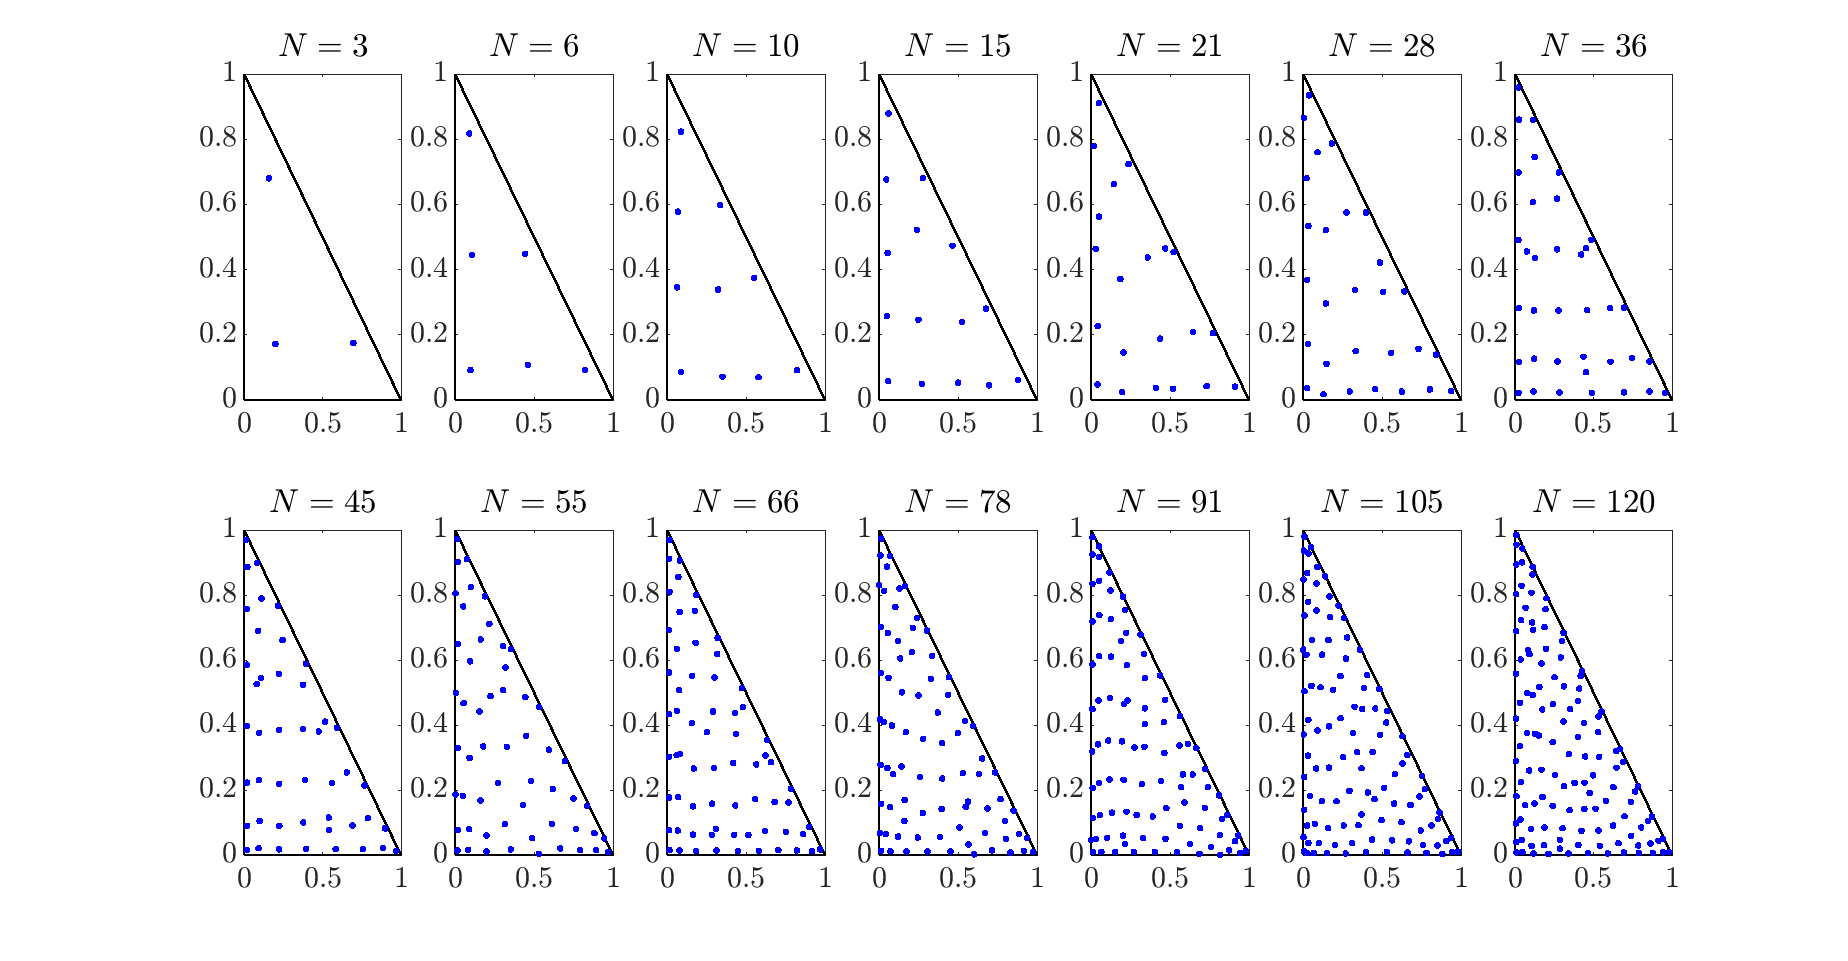
\includegraphics[width=1\linewidth]{./figures/triquadLeg_plot}
	\caption{Quadrature nodes on $\Tref^2$, corresponding to Table \ref{tab:quadverif}}\label{fig:triquadlegplot}
\end{figure}
In \myref{Figure}{fig:triquadlegerr}, we plot the relative error in approximating $I = \int_{\Tref^2} f(x,y) dxdy$ as $N$ the size of the quadrature rule is increased. The reference integrals $I$ are approximated with the quadrature rule of order $m=26$ (last column in \myref{Table}{tab:quadverif}).
\begin{figure}[H]
	\centering
	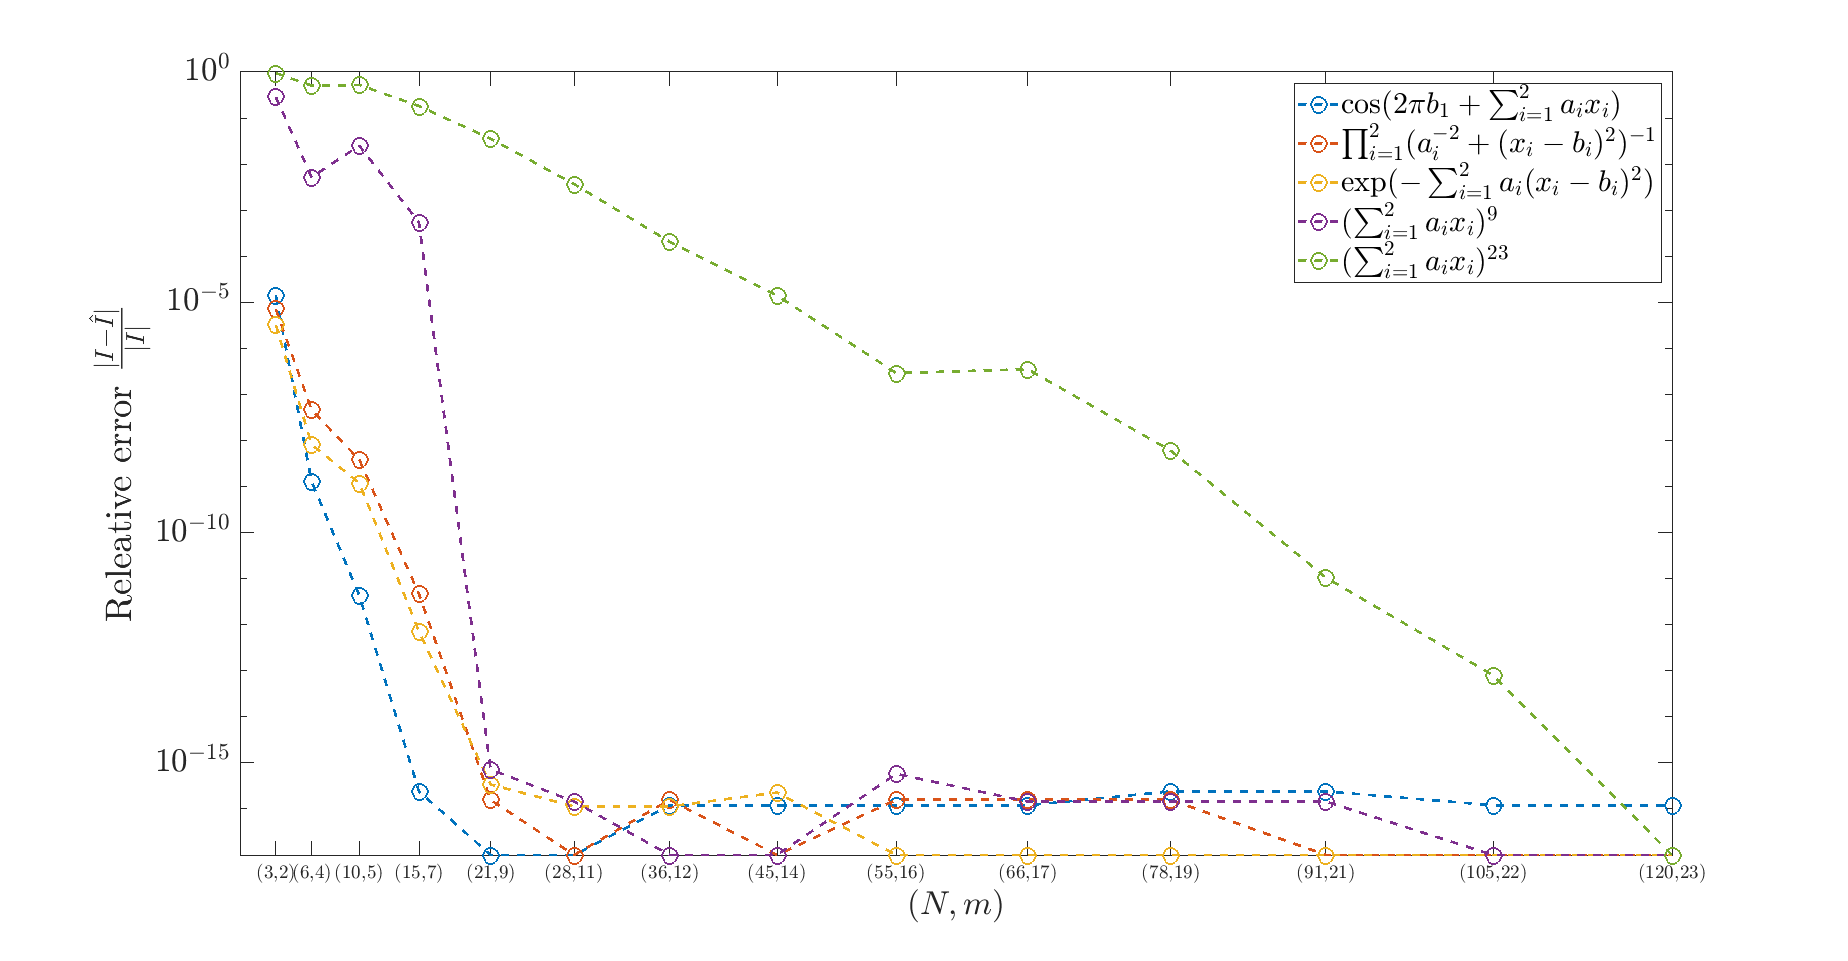
\includegraphics[width=0.9\linewidth]{./figures/triquadLeg_err}
	\caption{Relative error for integrating several test functions, including some of those due to \cite{genz}, as a function of the number of quadrature nodes $N$ and quadrature order $m$.}\label{fig:triquadlegerr}
\end{figure}

We choose several standard test functions, including a few due to Genz \cite{genz}. The function parameters $\bs{a},\bs{b} \in \bb{R}^2$ are drawn from the standard normal distribution. Polynomials of total degree $k$ are seen to be integrated to near machine precision by quadrature rules of order $m \geq k$. The rules are stable as $(N,m)$ are increased. Moreover, the decay is at least linear on a scale logarithmic only in $y$, which implies that the rules exhibit spectral convergence for these functions. 

Though not provided here, these results hold for alternative choices of $(a,b,c)$. However, the interpolation matrices tend to slowly grow more ill-conditioned as $(N,a,b,c)$ are increased, and it becomes more difficult for our algorithm to find suitable quadratures. To the extent that these quadratures are used for computing expansion coefficients, this is not a problem. We can always convert coefficients from the Legendre basis to one with larger parameters (integer difference), as described in \myref{Section}{sec:promotetri}.

\mysssection{Generalization for higher dimensions}{}
On the triangle, and in fact, for most higher dimensional orthogonal polynomials, $J_{n,i}$ are not exactly jointly diagonlizable. We exploited the isomorphism between $\bb{R}^2$ and the complex plane for $d=2$ to match the eigenvalues of $J_{n,1},J_{n,2}$. This structure does not exist for $d>2$. However, there is still a connection between the approximate joint eigenvalues of $J_{n,i}$ and interior points of $\Tref^2$. To be clear, we must specify what is meant by ``approximate'' joint eigenvalues. 

The approximate joint diagonalization problem for a set of real-valued symmetric matrices $\{C^1,\cdots,C^d\}$ is to find the orthogonal matrix $U$ such that the matrices 
\begin{equation}
	F^k = UC^kU^T, \quad 1\leq k \leq d
\end{equation}
are approximately diagonal. Alternatively, we can find the diagonal matrices $F^k$ such that $C^k$ are approximately equal to $U^TF^kU$. The definition of ``as diagonal as possible'' leads to various formulations of the diagonalization problem in terms of minimizing an objective function. For example, solving
\begin{equation}
	\min_{\substack{\text{$U\in \bb{R}^N$},\\ \text{$U^TU=UU^T=I$}}}\sum_{i\neq j}(F^k_{ij})^2
\end{equation}
is equivalent to minimizing the off-diagonal entries of $F^k$ by orthogonal similarity transformations of $C^k$. On the other hand, solving
\begin{equation}
	\min_{\substack{\text{$U,F^1,\cdots F^d$},\\ \text{$U^TU=UU^T=I$}}} \sum_{k=1}^d \big|\big|C^k-U^TF^k U\big|\big|_F^2
\end{equation}
is finding the best representation of $C^k$ in the basis of $U$ - a subspace fitting approach. For both problems, we require orthogonality of $U$, as we want it to represent the ``average eigenstructure" of $C^k$. For the Jacobi matrices $J_{n,i}$, this requirement is natural. We want a decomposition close to the optimal quadrature case of exact joint diagonlization. In fact, (I tested this using the methods described in \cite{bss} and \cite{jevd}) if the orthogonality requirement is removed, the eigenvalues (diagonals of $F^k$) will not necessarily be contained in $\Tref^2$. \color{red} If we can show that, under some assumption of the diagonality measure and the orthogonality requirement for $U$, the resulting solution (if found) gives eigenvalues within $\Tref^2$ (or a more general convex space), then we have a nice way to bootstrap Netwon-like methods for adaptive quadrature in $d$ dimensions.\color{black} \emph{ This is how we can generalize the Vioreanu-Rokhlin quadrature to 3D}.
%\color{blue}In the context of the HPS method, we investigated partitioning triangles into quadrilaterals, and using product orthogonal polynomials bases on each quad. Spectral convergence was observed for both integration as well as the solve - this might be the cleanest way forward.\color{black}

%On the other hand, we know that any quadrature rule capable of exactly integrating polynomials of total degree $2n-1$ requires the number of points $N$ to be at least $\dim\Pi_{n-1}^d$. \color{red} A thought I had was to find all of the joint eigenvalues that do exist (it will be less than $N$), and compute the associated weights as usual with the generalized Golub-Welsch algorithm. Then, we fix these nodes and weights, iteratively add more nodes (which we consider fixed), and compute weights for these. \color{black} The resulting quadrature should be exact for polynomials of degree up to $2n-1$, but we now will require more than $N$ points. This follows from the fact that a minimal quadrature rule has $N$ points, and there are no minimal Gaussian quadrature rules on the triangle.
\newpage
\myssection{Ladder, lowering and promotion operators for Koornwinder polynomials}{sec:promotetri}
In 1D, we obtained promotion operators which could map coefficients under $P^{(a,b)}$ to those under $P^{(a+1,b+1)}$ for Jacobi polynomial $P^{(a,b)}$, and ladder operators for the derivatives. For the Koornwinder polynomials in 2D, there exist similar relationships (\cite{jacladder},\cite{sparsetri}). Simultaneous promotion is obtained by composing partial promotion operators, and differentiation composes partial ladder operators with promotion operators.

Suppose we have a Koornwinder polynomial expansion of $f(x,y)$; $$f(x,y) \approx \bs{P}^{(a,b,c)}(x,y)^T\bs{f}.$$

\mysssection{Promotion operators}{sec:promoteoptri}
There exist banded operators which allow us to increment the parameters of a Koornwinder polynomial by one. We can equivalently express the expansion as 
\begin{align*}
	f(x,y)
	&\approx \bs{P}^{(a+1,b,c)}(x,y)^T\mathcal{K}_{(a,b,c)}^{(a+1,b,c)}\bs{f} \\
	&\approx \bs{P}^{(a,b+1,c)}(x,y)^T\mathcal{K}_{(a,b,c)}^{(a,b+1,c)}\bs{f} \\
	&\approx \bs{P}^{(a,b,c+1)}(x,y)^T\mathcal{K}_{(a,b,c)}^{(a,b,c+1)}\bs{f},
\end{align*}
where $\mathcal{K}_{(a,b,c)}^{(a+i,b+j,c+k)}$ is the promotion operator which maps the coefficients $\bs{f}$ of $f(x,y)$ in the basis of $\bs{P}^{(a,b,c)}$ to those in the basis of $\bs{P}^{(a+i,b+j,c+k)}$. For example, to promote the coefficients of $\bs{f}$ from $\bs{P}^{(a,b,c)}$ to $\bs{P}^{(a+1,b+1,c+1)}$, we would construct \begin{equation}
	\mathcal{K}_{(a,b,c)}^{(a+1,b+1,c+1)} = \mathcal{K}_{(a,b+1,c+1)}^{(a+1,b+1,c+1)}\mathcal{K}_{(a,b,c+1)}^{(a,b+1,c+1)}\mathcal{K}_{(a,b,c)}^{(a,b,c+1)}
\end{equation}
The entries of the single-parameter promotion operator are given by the following relations of $P_{k,n}^{(a,b,c)}$, where $h_{k,n}^{(a,b,c)}$ are the normalization constants from \eqref{eq:koornwinder}:
\begin{align}
(2n+a+b+c+2)h_{k,n}^{(a,b,c)}P_{k,n}^{(a,b,c)} &= (n+k+a+b+c+2)h_{k,n}^{(a+1,b,c)}P_{k,n}^{(a+1,b,c)}\nonumber\\
&+(n+k+b+c+1)h_{k,n-1}^{(a+1,b,c)}P_{k,n-1}^{(a+1,b,c)}\label{eq:ka}\\
(2n+a+b+c+2)(2k+b+c+1)h_{k,n}^{(a,b,c)}P_{k,n}^{(a,b,c)} &= (n+k+a+b+c+2)(k+b+c+1)h_{k,n}^{(a,b+1,c)}P_{k,n}^{(a,b+1,c)}\nonumber \\
&-(n-k+a)(k+b+c+1)h_{k,n-1}^{(a,b+1,c)}P_{k,n-1}^{(a,b+1,c)}\nonumber\\
&+(k+c)(n+k+b+c+1)h_{k-1,n-1}^{(a,b+1,c)}P_{k-1,n-1}^{(a,b+1,c)}\nonumber\\
&-(k+c)(n-k+1)h_{k-1,n}^{(a,b+1,c)}P_{k-1,n}^{(a,b+1,c)}\label{eq:kb}\\
(2n+a+b+c+2)(2k+b+c+1)h_{k,n}^{(a,b,c)}P_{k,n}^{(a,b,c)} &= (n+k+a+b+c+2)(k+b+c+1)h_{k,n}^{(a,b,c+1)}P_{k,n}^{(a,b,c+1)}\nonumber\\
&-(n-k+a)(k+b+c+1)h_{k,n-1}^{(a,b,c+1)}P_{k,n-1}^{(a,b,c+1)}\nonumber\\
&-(k+b)(n+k+b+c+1)h_{k-1,n-1}^{(a,b,c+1)}P_{k-1,n-1}^{(a,b,c+1)}\nonumber\\
&+(k+b)(n-k+1)h_{k-1,n}^{(a,b,c+1)}P_{k-1,n}^{(a,b,c+1)}\label{eq:kc}
\end{align}
The band structures of the promotion matrices are visualized in \myref{Figure}{fig:promotemat} for expansion order $n=6$. Each promotion matrix is in $\bb{R}^{N\times N}$ where $N=\dim\Pi_{n}^2$. Note, $\mathcal{K}_{(a,b,c)}^{(a,b+1,c)}$ and $\mathcal{K}_{(a,b,c)}^{(a,b,c+1)}$ have the same structure.
\begin{figure}[H]
	\centering
	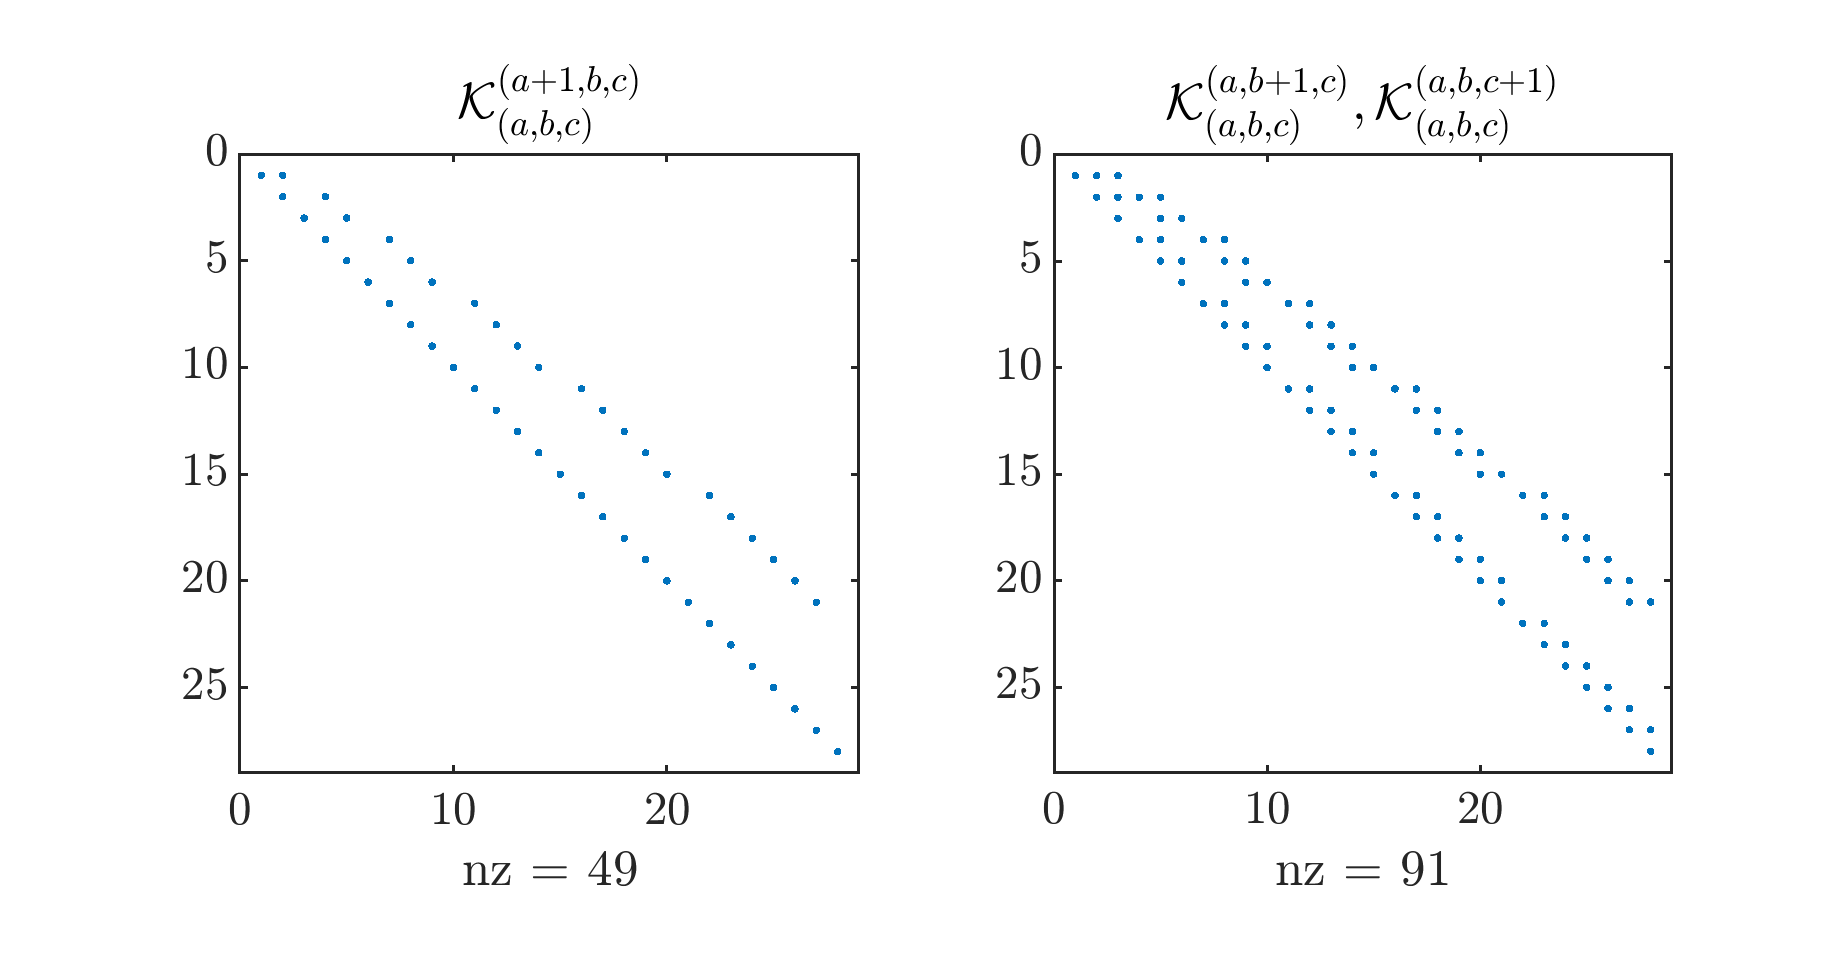
\includegraphics[width=1\linewidth]{./figures/promote_mat}
	\caption{Sparsity and band structure of the promotion matrices for $n=7$, $N=28$.}\label{fig:promotemat}
\end{figure}
To verify correctness of the implementation of these operators, we use the following procedure:
\begin{enumerate}[(i)]
\item Use the highest order quadrature available (last column of \myref{Table}{tab:quadverif}) to compute the coefficients of a function $f(x,y)$, as in \eqref{eq:jaccoeff}. That is, $$\bs{c} = \bs{P}^{(a,b,c)}(\bs{x},\bs{y})\big(f(\bs{x},\bs{y}) \odot \bs{w}\big)$$
\item Generate $K_{(a,b,c)}^{(a+1,b,c)},\mathcal{K}_{(a,b,c)}^{(a,b+1,c)},\mathcal{K}_{(a,b,c)}^{(a,b,c+1)}$ and compute $$\bs{c}_{a+1} = \mathcal{K}_{(a,b,c)}^{(a+1,b,c)}\bs{c},\s\s \bs{c}_{b+1} = \mathcal{K}_{(a,b,c)}^{(a,b+1,c)}\bs{c},\s\s \bs{c}_{c+1} = \mathcal{K}_{(a,b,c)}^{(a,b,c+1)}\bs{c}.$$
\item Check that $$||\bs{P}^{(a+1,b,c)}(\bs{x},\bs{y})\bs{c}_{a+1} - f(\bs{x},\bs{y})||,\s\s||\bs{P}^{(a,b+1,c)}(\bs{x},\bs{y})\bs{c}_{b+1} - f(\bs{x},\bs{y})||,\s\text{ and }||\bs{P}^{(a,b,c+1)}(\bs{x},\bs{y})\bs{c}_{c+1} - f(\bs{x},\bs{y})||$$ are near machine precision.
\end{enumerate}

\mysssection{Ladder operators}{}
Similar to 1D, there exist sparse relationships relating the partial derivatives of $P_{k,n}^{(a,b,c)}(x,y)$ to another Koornwinder polynomial with either the order $(n,k)$ or parameters $(a,b,c)$ incremented or decremented. In particular, the following recurrence relations can be used to construct partial derivatives to any order:
\begin{align}
(2k+b+c+1)h_{k,n}^{(a,b,c)}\partial_x P_{k,n}^{(a,b,c)} &= (n+k+a+b+c+2)(k+b+c+1)h_{k,n-1}^{(a+1,b,c+1)}P_{k,n-1}^{(a+1,b,c+1)} \nonumber \\
&+(k+b)(n+k+b+c+1)h_{k-1,n-1}^{(a+1,b,c+1)}P_{k-1,n-1}^{(a+1,b,c+1)},\label{eq:ladpartx}\\
h_{(k,n)}^{(a,b,c)}\partial_y P_{k,n}^{(a,b,c)} &= (k+b+c+1)h_{k-1,n-1}^{(a,b+1,c+1)}P_{k-1,n-1}^{(a,b+1,c+1)},\label{eq:ladparty}
\end{align}
so that there exist sparse banded matrices $\mathcal{D}_{x,(a,b,c)}^{(a+1,b,c+1)},\mathcal{D}_{y,(a,b,c)}^{(a,b+1,c+1)}$ such that
\begin{align}
	\partial_x f(x,y) \approx \partial_x \bs{P}^{(a,b,c)}(x,y)^T \bs{f} &= \bs{P}^{(a+1,b,c+1)}(x,y)^T\mathcal{D}_{x,(a,b,c)}^{(a+1,b,c+1)}\bs{f}\\
	\partial_y f(x,y) \approx \partial_y \bs{P}^{(a,b,c)}(x,y)^T \bs{f} &= \bs{P}^{(a,b+1,c+1)}(x,y)^T\mathcal{D}_{y,(a,b,c)}^{(a,b+1,c+1)}\bs{f}	
\end{align}
\mysssection{Weighted ladder operators}{}
The weighted basis $\tilde{\bs{P}}^{(a,b,c)}(x,y) = x^{a-\frac{1}{2}}y^{b-\frac{1}{2}}(1-x-y)^{c-\frac{1}{2}}\bs{P}^{(a,b,c)}$ will prove useful for incorporating boundary conditions to the discrete operator, while preserving its sparsity. This is accomplished using the following weighted ladder operators corresponding to differentiation of the weighted basis:
\begin{align}
	-(2k+b+c+1)h_{k,n}^{(a,b,c)}\partial_x\tilde{P}_{k,n}^{(a,b,c)} &=  (k+c)(n-k+1)h_{k,n+1}^{(a-1,b,c-1)}\tilde{P}_{k,n+1}^{(a-1,b,c-1)} \nonumber \\&+ (k+1)(n-k+a)h_{k+1,n+1}^{(a-1,b,c-1)}\tilde{P}_{k+1,n+1}^{(a-1,b,c-1)}\\
	h_{k,n}^{(a,b,c)}\partial_y\tilde{P}_{k,n}^{(a,b,c)} &= -(k+1)h_{k+1,n+1}^{(a,b-1,c-1)}\tilde{P}_{k+1,n+1}^{(a,b-1,c-1)}.
\end{align}
If $\bs{f}$ are the coefficients of $f$ under the weighted basis, then we have sparse banded matrices $\mathcal{W}_{x,(a,b,c)}^{(a-1,b,c-1)},\mathcal{W}_{y,(a,b,c)}^{(a,b-1,c-1)}$ such that
\begin{align}
	\partial_x f(x,y) = \partial_x (\tilde{\bs{P}}^{(a,b,c)}(x,y)^T\bs{f}) &= \tilde{\bs{P}}^{(a-1,b,c-1)}(x,y)^T \mathcal{W}_{x,(a,b,c)}^{(a-1,b,c-1)}\bs{f},\\
	\partial_y f(x,y) = \partial_y (\tilde{\bs{P}}^{(a,b,c)}(x,y)^T\bs{f}) &= \tilde{\bs{P}}^{(a,b-1,c-1)}(x,y)^T \mathcal{W}_{y,(a,b,c)}^{(a,b-1,c-1)}\bs{f}
\end{align}
\mysssection{Lowering operators}{}
Additionally, we have lowering operators which relate $xP_{k,n}^{(a,b,c)}$ to $P_{k,n}^{(a-1,b,c)}$ and $yP_{k,n}^{(a,b,c)}$ to $P_{k,n}^{(a,b-1,c)}$. These are given by the following recurrences:
\begin{align}
(2n+a+b+c+2)h_{k,n}^{(a,b,c)}xP_{k,n}^{(a,b,c)} &= (n-k+a)h_{k,n}^{(a-1,b,c)}P_{k,n}^{(a-1,b,c)} + (n-k+1)h_{k,n+1}^{(a-1,b,c)}P_{k,n+1}^{(a-1,b,c)},\\
(2k+b+c+1)(2n+a+b+c+2)h_{k,n}^{(a,b,c)}yP_{k,n}^{(a,b,c)} &= (k+b)(n+k+b+c+1)h_{k,n}^{(a,b-1,c)}P_{k,n}^{(a,b-1,c)} \nonumber \\
&-(k+1)(n-k+a)h_{k+1,n}^{(a,b-1,c)}P_{k+1,n}^{(a,b-1,c)} \nonumber \\
&-(k+b)(n-k+1)h_{k,n+1}^{(a,b-1,c)}P_{k,n+1}^{(a,b-1,c)} \nonumber \\
&+(k+1)(n+k+a+b+c+2)h_{k+1,n+1}^{(a,b-1,c)}P_{k+1,n+1}^{(a,b-1,c)}.
\end{align}
So, there are sparse banded matrices $\mathcal{L}_{(a,b,c)}^{(a-1,b,c)}$ and $\mathcal{L}_{(a,b,c)}^{(a,b-1,c)}$ corresponding to multiplication by $x$ and $y$, respectively, such that
\begin{align}
	xf(x,y) &= x\bs{P}^{(a,b,c)}(x,y)^T\bs{f} = \bs{P}^{(a-1,b,c)}(x,y)^T\mathcal{L}_{(a,b,c)}^{(a-1,b,c)}\bs{f},\\
	yf(x,y) &= x\bs{P}^{(a,b,c)}(x,y)^T\bs{f} = \bs{P}^{(a,b-1,c)}(x,y)^T\mathcal{L}_{(a,b,c)}^{(a,b-1,c)}\bs{f}.
\end{align}
\myssection{Sparse partial differential operator on $\Tref^2$}{}
In order to combine the discrete partial derivative operators into the Laplacian, we must promote the coefficients of the derivatives so that they are coordinates in the same basis. To be clear, we have
\begin{align*}
	\partial_{xx}f(x,y) &\approx \partial_x\big(\partial_x \bs{P}^{(a,b,c)}(x,y)^T\bs{f}\big) \\
	&= \partial_x\Big(\bs{P}^{(a+1,b,c+1)}(x,y)^T \mathcal{D}_{x,(a,b,c)}^{(a+1,b,c+1)}\bs{f}\Big) \\
	&= \bs{P}^{(a+2,b,c+2)}(x,y)^T\mathcal{D}_{x,(a+1,b,c+1)}^{(a+2,b,c+2)}\mathcal{D}_{x,(a,b,c)}^{(a+1,b,c+1)}\bs{f}\\
	\partial_{yy}f(x,y) &\approx \partial_y\big(\partial_y \bs{P}^{(a,b,c)}(x,y)^T\bs{f}\big) \\
	&= \partial_y\Big(\bs{P}^{(a,b+1,c+1)}(x,y)^T \mathcal{D}_{y,(a,b,c)}^{(a,b+1,c+1)}\bs{f}\Big) \\
	&= \bs{P}^{(a,b+2,c+2)}(x,y)^T\mathcal{D}_{y,(a,b+1,c+1)}^{(a,b+2,c+2)}\mathcal{D}_{y,(a,b,c)}^{(a,b+1,c+1)}\bs{f}\\
	\partial_{xy}f(x,y) &\approx \partial_x\big(\partial_y \bs{P}^{(a,b,c)}(x,y)^T\bs{f}\big) \\
&= \partial_x\Big(\bs{P}^{(a,b+1,c+1)}(x,y)^T \mathcal{D}_{y,(a,b,c)}^{(a,b+1,c+1)}\bs{f}\Big) \\
&= \bs{P}^{(a+1,b+1,c+2)}(x,y)^T\mathcal{D}_{x,(a,b+1,c+1)}^{(a+1,b+1,c+2)}\mathcal{D}_{y,(a,b,c)}^{(a,b+1,c+1)}\bs{f}
\end{align*}  
Since the coefficients of $\partial_{xx}f(x,y)$ are in the span of $\bs{P}^{(a+2,b,c+2)}$, while those of $\partial_{yy}f(x,y)$ are in the span of $\bs{P}^{(a,b+2,c+2)}$, we can promote both of them to $(a+2,b+2,c+2)$. Let $\Delta_{(a,b,c)}^{(a+2,b+2,c+2)}$ denote the discrete Laplacian which takes the modes of $f(x,y)$ in the basis of $\bs{P}^{(a,b,c)}$ and returns the coefficients of $\Delta f$ in the basis of $\bs{P}^{(a+2,b+2,c+2)}$. Then, we can construct the modal operator through
\begin{equation}\label{eq:laptrimat}
	\begin{split}
	\Delta_{(a,b,c)}^{(a+2,b+2,c+2)} &= \mathcal{K}_{(a+2,b+1,c+2)}^{(a+2,b+2,c+2)}\mathcal{K}_{(a+2,b,c+2)}^{(a+2,b+1,c+2)}\mathcal{D}_{x,(a+1,b,c+1)}^{(a+2,b,c+2)}\mathcal{D}_{x,(a,b,c)}^{(a+1,b,c+1)}\\
	&+\mathcal{K}_{(a+1,b+2,c+2)}^{(a+2,b+2,c+2)}\mathcal{K}_{(a,b+2,c+2)}^{(a+1,b+2,c+2)}\mathcal{D}_{y,(a,b+1,c+1)}^{(a,b+2,c+2)}\mathcal{D}_{y,(a,b,c)}^{(a,b+1,c+1)}
	\end{split}
\end{equation}

All operators have been verified using a similar approach to that presented at the end of \myref{Section}{sec:promoteoptri}. To eliminate the rank deficiency in the modal Laplacian and construct an operator which will solve \eqref{eq:laptri}, we can use properties (i)-(iii) listed in \myref{Section}{sec:koornpoly}. By evaluating the polynomials on the boundary, we can explicitly enforce the boundary conditions. For expansion order $m-1$, we always have $$\text{rank}\big(\Delta_{(a,b,c)}^{(a+2,b+2,c+2)}\big) = (m-2)(m-1)/2.$$ So, there are $m(m+1)/2-(m-2)(m-1)/2 = 2m-1$ rank deficient rows. To fill in the rank deficient rows with the boundary conditions, we must first select the appropriate number of interpolation nodes for the left, bottom and hypotenuse edge of $\Tref^2$. 
\begin{itemize}
	\item For the left and bottom edges, we take $$N_\text{lb} = \Big\lfloor \frac{2m-1}{2+\sqrt{2}} \Big\rfloor.$$
	\item For the hypotenuse, we take $$N_{\text{h}} = (2m-1)-2N_{\text{lb}}.$$
\end{itemize}

The nodes for this task come from three 1D Gauss-Jacobi quadrature rules with parameters $a,b$. For example, the complete operator with Dirichlet boundary conditions can be given as 
 \begin{equation}
 \tilde{\Delta}_{(a,b,c)}^{(a+2,b+2,c+2)} = \begin{bmatrix}\Delta_{(a,b,c)}^{(a+2,b+2,c+2)} \\
 \bs{P}^{(a,b,c)}(\bs{x}_b,0)^T\\
 \bs{P}^{(a,b,c)}(0,\bs{x}_l)^T\\
 \bs{P}^{(a,b,c)}(\bs{x}_h,1-\bs{x}_h)^T\end{bmatrix},
 \end{equation}
where $\bs{x}_b,\bs{x}_l$ and $\bs{x}_h$ are Gauss-Jacobi nodes shifted to the interval $(0,1)$ for the bottom, left and hypotenuse edges of $\Tref^2$. The process for solving \eqref{eq:laptri} is then as follows:
\begin{enumerate}[(i)]
	\item Expand the right-hand side $f(x,y)$ in the basis $\bs{P}^{(\frac{3}{2},\frac{3}{2},\frac{3}{2})}$ by first computing the coefficients in $\bs{P}^{(\frac{1}{2},\frac{1}{2},\frac{1}{2})}$ and promoting them by composing the three single-parameter promotion matrices. 
	\item Assemble $\tilde{\Delta}$ and solve for the coefficients $\bs{u}$ of $u(x,y)$ in the basis $\bs{P}^{(\frac{1}{2},\frac{1}{2},\frac{1}{2})}$ through $$\bs{u} = \tilde{\Delta}^{-1}\begin{bmatrix}\bs{f}\\
	g(\bs{x_b},0)^T\\g(0,\bs{x_l})^T\\g(\bs{x}_h,1-\bs{x}_h)^T\end{bmatrix},$$ where $\bs{f}$ are the coefficients of the right-hand side under $\bs{P}^{(\frac{3}{2},\frac{3}{2},\frac{3}{2})}$ obtained in step (i).
	\item Evaluate the approximation $\hat{u}(x,y)$ using the Vandermonde matrix as $$\hat{u}(\bs{x},\bs{y}) = \bs{P}^{(\frac{1}{2},\frac{1}{2},\frac{1}{2})}(\bs{x},\bs{y})^T\bs{u},$$ where $\bs{x},\bs{y}$ are the quadrature nodes used in step (i).
\end{enumerate}


For the case of zero Dirichlet boundary conditions, we can use the weighted basis $\tilde{\bs{P}}^{(a,b,c)}$ which evaluates to $\bs{0}$ on the boundary and naturally satisfies homogeneous Dirichlet conditions. We will construct the modal Laplacian $\Delta_W$ which operates on coefficients under the basis $\tilde{\bs{P}}^{(3/2,3/2,3/2)}$ and produces coefficients under $\bs{P}^{(3/2,3/2,3/2)}$. Note, \emph{the conversion from the weighted to regular Koornwinder basis depends on our choice of parameters $a=b=c=3/2$}. 

With $\bs{f}$ the coefficients of $f(x,y)$ in the weighted basis, 
\begin{align*}
	\partial_x f(x,y) &= \tilde{\bs{P}}^{a-1,b,c-1}(x,y)^T \mathcal{W}_{x,(a,b,c)}^{(a-1,b,c-1)}\bs{f} \\
	& = x^{a-\frac{3}{2}}y^{b-\frac{3}{2}}(1-x-y)^{c-\frac{3}{2}}\big(y\bs{P}^{(a-1,b,c-1)}(x,y)\big)^T(\mathcal{W}_{x,(a,b,c)}^{(a-1,b,c-1)}\bs{f})\\
	&= x^{a-\frac{3}{2}}y^{b-\frac{3}{2}}(1-x-y)^{c-\frac{3}{2}}\bs{P}^{(a-1,b-1,c-1)}(x,y)^T(\mathcal{L}_{(a-1,b,c-1)}^{(a-1,b-1,c-1)}\mathcal{W}_{x,(a,b,c)}^{(a-1,b,c-1)}\bs{f}),\\
	\partial_y f(x,y) &= \tilde{\bs{P}}^{(a,b-1,c-1)}(x,y)^T \mathcal{W}_{y,(a,b,c)}^{(a,b-1,c-1)}\bs{f} \\
	&= x^{a-\frac{3}{2}}y^{b-\frac{3}{2}}(1-x-y)^{c-\frac{3}{2}}\big(x\bs{P}^{(a,b-1,c-1)}(x,y)\big)^T(\mathcal{W}_{y,(a,b,c)}^{(a,b-1,c-1)}\bs{f})\\
	&=x^{a-\frac{3}{2}}y^{b-\frac{3}{2}}(1-x-y)^{c-\frac{3}{2}}\bs{P}^{(a-1,b-1,c-1)}(x,y)^T(\mathcal{L}_{(a,b-1,c-1)}^{(a-1,b-1,c-1)}\mathcal{W}_{y,(a,b,c)}^{(a,b-1,c-1)}\bs{f})
\end{align*}
When $a=b=c=3/2$, we have 
\begin{align*}
	\partial_x f(x,y) &=  \bs{P}^{(a-1,b-1,c-1)}(x,y)^T(\mathcal{L}_{(a-1,b,c-1)}^{(a-1,b-1,c-1)}\mathcal{W}_{x,(a,b,c)}^{(a-1,b,c-1)}\bs{f}),\\
\partial_yf(x,y) &= \bs{P}^{(a-1,b-1,c-1)}(x,y)^T(\mathcal{L}_{(a,b-1,c-1)}^{(a-1,b-1,c-1)}\mathcal{W}_{y,(a,b,c)}^{(a,b-1,c-1)}\bs{f}),
\end{align*}
so that the second partials can be constructed with the promotion and unweighted ladder operator:
\begin{align}
	\partial_{xx}f(x,y) &= \bs{P}^{(a,b,c)}(x,y)^T\Big( \mathcal{K}_{(a,b-1,c)}^{(a,b,c)}\mathcal{D}_{x,(a-1,b-1,c-1)}^{(a,b-1,c)}\mathcal{L}_{(a-1,b,c-1)}^{(a-1,b-1,c-1)}\mathcal{W}_{x,(a,b,c)}^{(a-1,b,c-1)}\bs{f}\Big),\\
	\partial_{yy}f(x,y) &= \bs{P}^{(a,b,c)}(x,y)^T\Big( \mathcal{K}_{(a-1,b,c)}^{(a,b,c)}\mathcal{D}_{y,(a-1,b-1,c-1)}^{(a-1,b,c)}\mathcal{L}_{(a,b-1,c-1)}^{(a-1,b-1,c-1)}\mathcal{W}_{y,(a,b,c)}^{(a,b-1,c-1)}\bs{f}\Big),\\
	\partial_{xy}f(x,y) &= \bs{P}^{(a,b,c)}(x,y)^T\Big(\mathcal{K}_{(a,b-1,c)}^{(a,b,c)}\mathcal{D}_{x,(a-1,b-1,c-1)}^{(a,b-1,c)}\mathcal{L}_{(a,b-1,c-1)}^{(a-1,b-1,c-1)}\mathcal{W}_{y,(a,b,c)}^{(a,b-1,c-1)}\bs{f}\Big)
\end{align}
$\Delta_W$ is then given by
\begin{equation}\label{eq:laptriweight}
	 \begin{split}
	\Delta_W	&= \mathcal{K}_{(a,b-1,c)}^{(a,b,c)}\mathcal{D}_{x,(a-1,b-1,c-1)}^{(a,b-1,c)}\mathcal{L}_{(a-1,b,c-1)}^{(a-1,b-1,c-1)}\mathcal{W}_{x,(a,b,c)}^{(a-1,b,c-1)} \\
	&+\mathcal{K}_{(a-1,b,c)}^{(a,b,c)}\mathcal{D}_{y,(a-1,b-1,c-1)}^{(a-1,b,c)}\mathcal{L}_{(a,b-1,c-1)}^{(a-1,b-1,c-1)}\mathcal{W}_{y,(a,b,c)}^{(a,b-1,c-1)}
	\end{split}
\end{equation}
The matrix $\Delta_W$ has full rank, as indicated by the fill-in the last rows and columns of the sparsity pattern in \myref{Figure}{fig:laptrimat1}. The process for solving \eqref{eq:laptri} with zero Dirichlet conditions is as follows:
\begin{enumerate}[(i)]
	\item Expand the right-hand side $f(x,y)$ in the basis $\bs{P}^{(\frac{3}{2},\frac{3}{2},\frac{3}{2})}$ by first computing the coefficients in $\bs{P}^{(\frac{1}{2},\frac{1}{2},\frac{1}{2})}$ and promoting them by composing the three single-parameter promotion matrices. 
	\item Assemble $\Delta_W$ and solve for the coefficients $\bs{u}$ of $u(x,y)$ in the weighted basis $\tilde{\bs{P}}^{(\frac{3}{2},\frac{3}{2},\frac{3}{2})}$ through $$\bs{u} = \Delta_W^{-1}\bs{f},$$ where $\bs{f}$ are the coefficients of the right-hand side under $\bs{P}^{(\frac{3}{2},\frac{3}{2},\frac{3}{2})}$ obtained in step (i).
	\item Evaluate the approximation $\hat{u}(x,y)$ using the weighted Vandermonde matrix as $$\hat{u}(\bs{x},\bs{y}) = \tilde{\bs{P}}^{(\frac{3}{2},\frac{3}{2},\frac{3}{2})}(\bs{x},\bs{y})^T\bs{u},$$ where $\bs{x},\bs{y}$ are the quadrature nodes used in step (i).
\end{enumerate}

\begin{figure}[H]
	\centering
	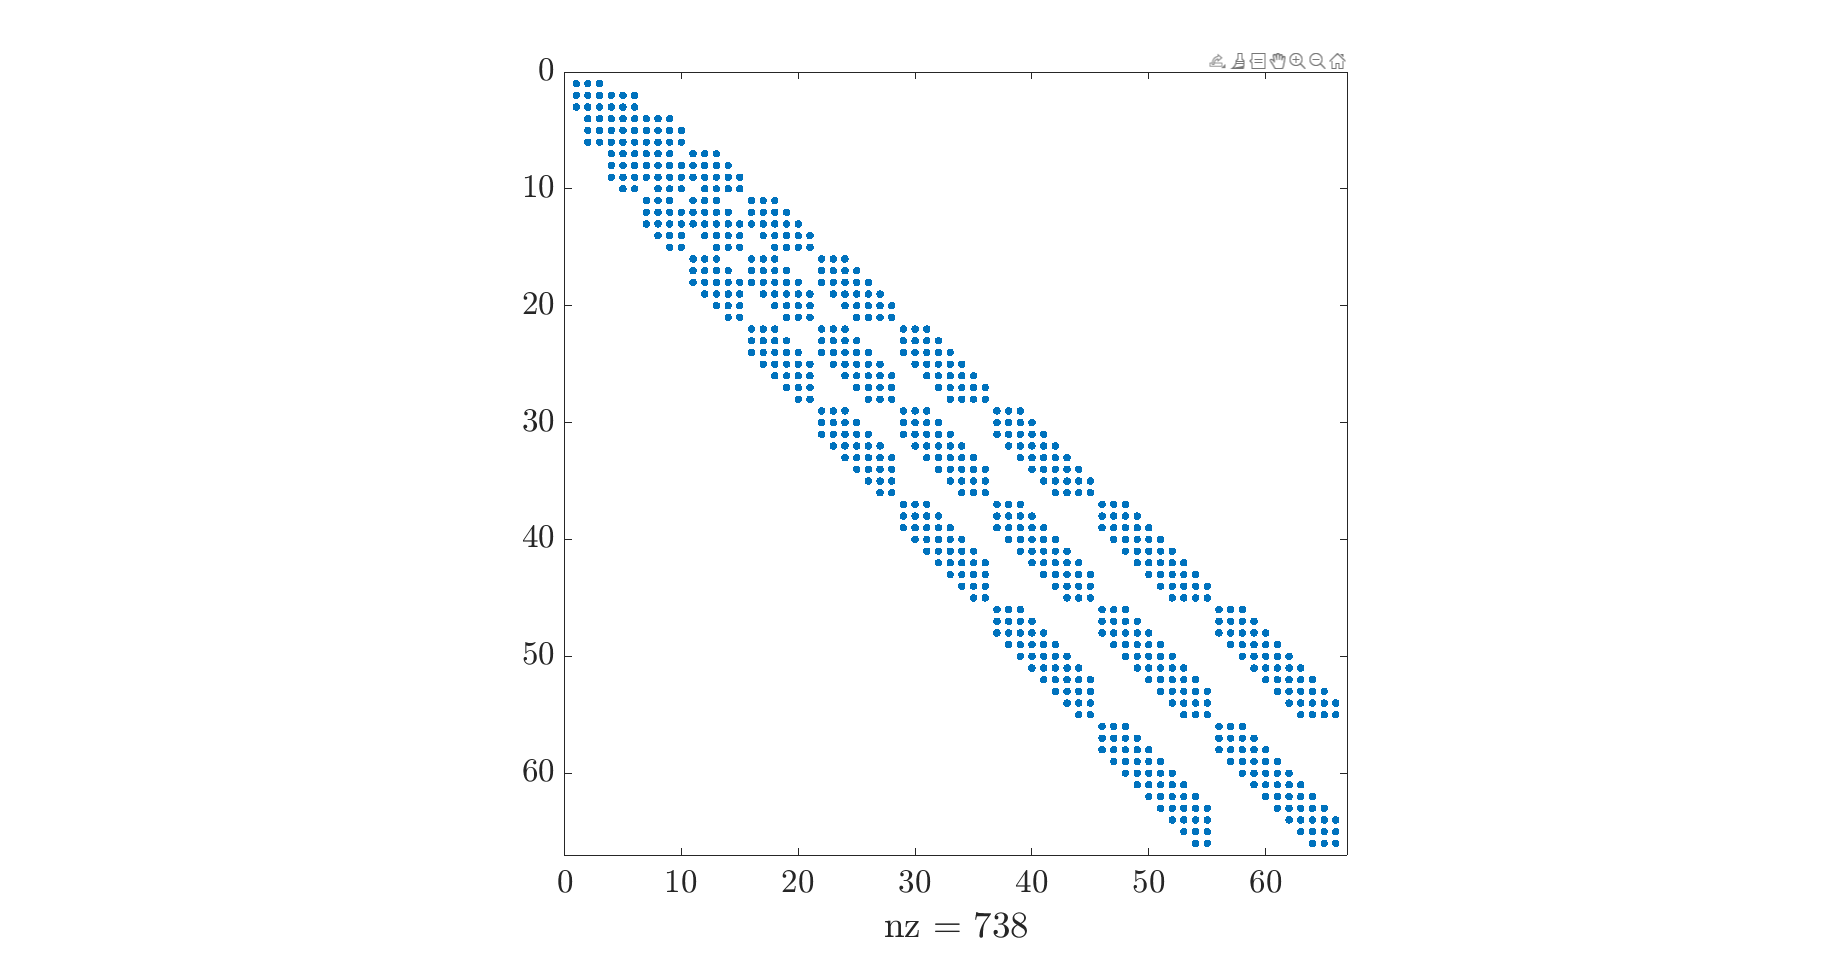
\includegraphics[width=1\linewidth]{./figures/lap_tri_weighted_mat}
	\caption{Sparsity and band structure of the weighted modal Laplacian \eqref{eq:laptriweight} for expansion order $n=13$.}\label{fig:laptrimat1}
\end{figure}

\myssection{Sparse partial differential operator on general $\Tau^2$}{}
For general triangular elements $\Tau^2$ with vertices $(x_0,y_0),(x_1,y_1), (x_2,y_2)$, we can use the following affine transformation for $x,y\in\Tau^2$ and $r,s\in \Tref^2$ to construct a map between $\Tau^2$ and $\Tref^2$;
\begin{align}
\begin{bmatrix}
r\\
s
\end{bmatrix} &\mapsto
A
\begin{bmatrix} r\\s\end{bmatrix} + 
\begin{bmatrix}
x_0\\
y_0
\end{bmatrix} = \begin{bmatrix} x \\ y \end{bmatrix},\label{duffygen}\\
\begin{bmatrix}
x\\
y
\end{bmatrix} &\mapsto A^{-1}\begin{bmatrix}
x-x_0\\
y-y_0
\end{bmatrix} = \begin{bmatrix}
r\\
s
\end{bmatrix},\label{duffygeninv}
\end{align}
where 
\begin{equation*}
A = \begin{bmatrix}
x_1-x_0 & x_2-x_0\\
y_1-y_0 & y_2-y_0
\end{bmatrix}.
\end{equation*}
For $(x,y)\in\Tau^2$, the Laplacian is augmented with Jacobian factors of the coordinate transformation:
\begin{align}
\partial_{xx} u &= (\partial_x r)^2(\partial_{rr}u) + 2(\partial_x r)(\partial_x s)(\partial_{rs}u) + (\partial_x s)^2 (\partial_{ss}u) + (\partial_{xx} r)(\partial_r u) + (\partial_{xx} s)(\partial_s u)\nonumber\\
&= (\partial_x r)^2(\partial_{rr}u) + 2(\partial_x r)(\partial_x s)(\partial_{rs}u) + (\partial_x s)^2 (\partial_{ss}u),\label{dxxmap}\\
\partial_{yy} u &= (\partial_y r)^2(\partial_{rr}u) + 2(\partial_y r)(\partial_y s)(\partial_{rs}u) + (\partial_y s)^2 (\partial_{ss}u) + (\partial_{yy} r)(\partial_r u) + (\partial_{yy} s)(\partial_s u)\nonumber\\
&=(\partial_y r)^2(\partial_{rr}u) + 2(\partial_y r)(\partial_y s)(\partial_{rs}u) + (\partial_y s)^2 (\partial_{ss}u) \label{dyymap},
\end{align}
from which we note we have to additionally compute the modal mixed partial operator $\mathcal{D}_{rs}$. 

\textbf{Note}: We find that the condition number of the discrete operator with boundary conditions included is best controlled if the boundary nodes are distributed to the edges of $\mathcal{T}^2$ according to length fraction. In this way, longer sides get more nodes, and smaller sides get fewer. This avoids node coalescence when aspect ratio is large.

\myssection{Numerical experiments}{}
In \myref{Figure}{fig:errslapweight}, we plot the relative solution error in solving \eqref{eq:laptri} for several manufactured solutions (see the legend) satisfying the homogeneous Dirichlet B.C. $g(x,y)=0$ on the reference triangle $\Tref^2$. In the figure, $N = \dim\Pi_{n}^d = (n+1)(n+2)/2$ is the number of coefficients, and $n$ is the expansion order. For each problem considered, we obtain at least one digit of accuracy as the expansion order $n$ is increased by one. Hence, the method and implementation exhibits spectral convergence.
\begin{figure}[H]
	\centering
	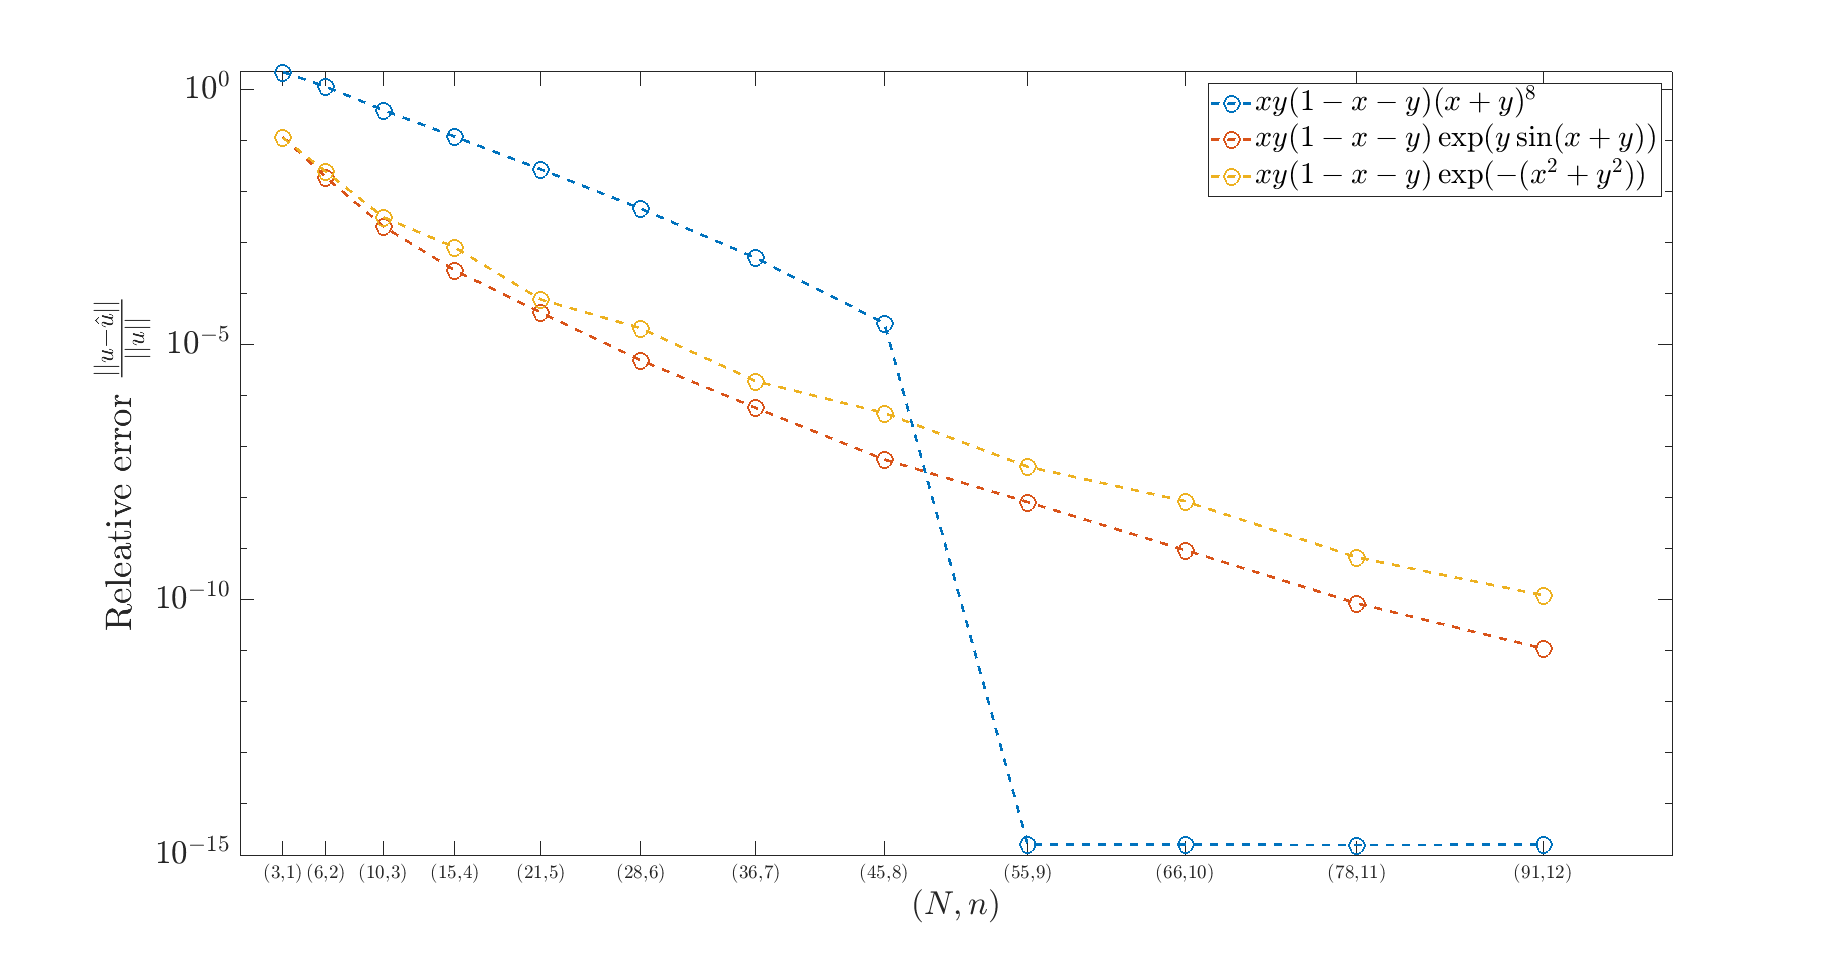
\includegraphics[width=0.75\linewidth]{./figures/errs_lap_weight}
	\caption{Relative error in solving \eqref{eq:laptri} for several manufactured solutions $u$ (see legend) with $g(x,y) = 0$ (homogeneous Dirichlet B.Cs) as the expansion order is increased}\label{fig:errslapweight}
\end{figure}

Now, we will consider a range of increasingly degenerate triangles by sampling the $y_3$ coordinate from $[0.001,1]$ corresponding to aspect ratios between $[1,500]$. That is, we shift the top corner of the reference triangle down, making each subsequent triangle thinner. We want to know how the methods (unweighted vs weighted) are affected by the aspect ratio of the triangle. In \myref{Figure}{fig:errslapaspect}, we plot the relative error in the solution to \eqref{eq:laptri} on several (non-reference) triangles $\mathcal{T}$ with aspect ratios between $[1,500]$. We see that for the entire range of aspect ratios considered (very thin to normal triangles), both methods exhibit spectral convergence. The inset panels show the dependence of the conditioning of the discrete operator on the aspect ratio for a fixed order. We see that the operator grows illconditioned as the aspect ratio increases. This growth is better controlled in the weighted case.

\begin{figure}[H]
	\centering
	\includegraphics[width=1\linewidth]{./figures/errs_lap_aspect}
	\caption{Relative error in solving \eqref{eq:laptri} for several manufactured solutions $u$ (see legend) with boundary condition $g(x,y) = u(x,y)$ for the unweighted Laplacian and $g(x,y)=0$ for the weighted one as the expansion order is increased. Several aspect ratios between $[1,500]$ are considered.}\label{fig:errslapaspect}
\end{figure}
In \myref{Figure}{fig:lapcond}, we plot the condition number of the discrete operator as the expansion order is increased, for each aspect ratio and the weighted/unweighted methods. The weighted basis gives a much better conditioned operator, though both methods exhibit growth of the condition number in $N$. The width of the bands indicates control given a fixed $N$ and growth in aspect ratio.

Hence, for the unweighted basis, to mitigate loss of accuracy as the aspect ratio increases, we need to find even better boundary nodes to keep the discrete operator reasonably conditioned as expansion order is increased. 


\begin{figure}[H]
	\centering
	\includegraphics[width=1\linewidth]{./figures/cond_lap}
	\caption{Condition number of weighted and unweighted discrete modal Laplacians for several expansion orders and aspect ratios.}\label{fig:lapcond}
\end{figure}

\newpage
\mysection{General theory of orthogonal polynomials}{sec:orthopoly}

In this section, we provide a general theory for orthogonal polynomials in 1D, and follow with the multivariable case. More details can be found in \cite{dunkl_xu}. Let $X \subset \bb{R}^{d\geq 1}$, $\mu$ a probability measure on $X$, and $\{f_i(x)\}_{i\geq 1}=\bs{f}(x)$ a set of linearly independent functions in $L^2(X,\mu)$ arranged as a column vector. Denote the weighted $L^2$ inner product as $\langle f, g \rangle = \int_{X} fg d\mu$. Recall, the projection of $g \in L^2(X,\mu)$ onto $\text{span}\{f_i\}$ involves solving equations of the form $(Ga)_i = \langle f,f_i\rangle$, where $G$ is the Gram matrix.

\begin{definition}\normalfont
For linearly independent $\{f_i(x)\}_{i\geq 1} \in L^2(X,\mu)$, the \underline{Gram matrix} $G$ has entries
	$$g_{ij} = \langle f_i,f_j\rangle.$$
\end{definition}

\begin{definition}\label{def:moments}\normalfont
For some $n\in\bb{N}$, let the \underline{moment determinants} be given by
\begin{equation} 
d_n = \det{(g_{ij})_{i,j=1}^n},
\end{equation} 
with $d_0=1$, and define the polynomial $D_n(x)$ by
\begin{equation}
D_n(x) = \det{
	\begin{bmatrix} (g_{ij})_{i,j = 1}^{n-1,n} \\ \bs{f}(x)^T  \end{bmatrix}} 
\end{equation}
\end{definition}

\begin{proposition}\label{prop:moments}\normalfont
We make the following observations:
\begin{enumerate}[(i)]
	\item $\text{span}\{\big(D_j(x)\big)_{j=1}^n\} = \text{span}\{\big(f_j(x)\big)_{j=1}^n\}$
	\item The functions $\{D_n(x)\}$ are orthogonal in $L^2(X,\mu)$.
	\item $\langle D_n,D_n\rangle = d_nd_{n-1}$.
\end{enumerate}
\end{proposition}
\begin{proof}
Observe that for some $v \in \bb{R}^n$,
$$ v^T G v = \int_{X} v^T \bs{f}\bs{f}^T v d\mu = \int_{X} ||\bs{f}^Tv||_2^2 d\mu \geq 0.$$
Since $\bs{f} = \{f_j\}_{j=1}^n$ are linearly independent, we can only have equality above if $v = 0$. Hence, $G \succ 0$, and $d_n = \det(G) > 0$. By method of minors, $D_n(x) = d_{n-1}f_n(x) + \sum_{j < n} c_j f_j(x)$ for principle minors $c_j$. Clearly, $\text{span}\{\big(D_j(x)\big)_{j=1}^n\} = \text{span}\{\big(f_j(x)\big)_{j=1}^n\}$. For orthogonality, note that $$\big\langle D_n,D_j\big\rangle = \big\langle D_n, d_{j-1}f_j + \sum_{k<n} c_k f_k\big\rangle = d_{j-1}\big\langle D_n,f_j\big\rangle+ \sum_{k<n}c_k\big\langle D_n,f_k\big\rangle.$$ Expanding $\langle D_n,f_j\rangle$, we see that $$\langle D_n,f_j\rangle = \det{
	\begin{bmatrix} (g_{ij})_{i,j = 1}^{n-1,n} \\ \int_{X}f_j\bs{f}(x)^Td\mu  \end{bmatrix}} = \det{
\begin{bmatrix} (g_{ij})_{i,j = 1}^{n-1,n} \\ (g_{jk})_{k=1}^n \end{bmatrix}} = d_n\delta_{jn},$$
since for $j < n$, the second block is a dependent row. Thus, we can eliminate the sum in the orthogonality relation, yielding $$\langle D_n,D_j\rangle = d_{j-1}d_n\delta_{jn}.$$
\end{proof}
\begin{definition}\normalfont
	Given a member $P_n(x)$ of a family of orthogonal polynomials, the \underline{structural constant} for $P_n$ is defined as
	\begin{equation}
	h_n = \int_a^b P_n(x)^2d\mu(x).
	\end{equation}
\end{definition}
\vspace{-10pt}
\myssection{Single variable}{}
Using the results from the previous section, we can now specialize to polynomials of a single variable $x \in [a,b]$. Let $\mu$ be a measure supported on $[a,b]$ with $\int_{X}|x|^n d\mu < \infty,\s \forall n$. Consider the monomial basis $\{x^{j-1}\}_{j\geq 1}$. The moment determinants are $$g_{ij} = c_{i+j-2},\quad c_n = \int_{a}^b x^n d\mu(x).$$ Since $\{D_n(x)\}$ generated with the monomial basis are orthogonal with structure factor $d_{n-1}d_n$, we can use them as our orthonormal polynomials. Let $P_{n\geq0}(x) = D_{n+1}(x)$. Then,
\begin{equation}
p_{n\geq 0}(x) = (d_nd_{n+1})^{-1/2}P_{n}(x).
\end{equation}

By construction $\langle p_n,q\rangle = 0$ for any $q \in \bb{P}_{k<n}$. Moreover, we can compute the \underline{leading coefficient} $k_n$ through \begin{equation}\label{eq:orthnormlead}
p_n(x)=(d_nd_{n+1})^{-1/2}\big(d_nx^n+ \sum_{j=1}^n a_jx^{j-1}\big)\Rightarrow k_n = (d_n/d_{n+1})^{1/2} > 0,
\end{equation}
where positivity of $k_n$ follows from the fact that $d_n > 0$ (leading coefficient of normalized polynomial has the same sign as the original). The process used here to generate $p_n$ is equivalent to applying the Gram-Schmidt process on the monomial basis with respect to the weight/measure $\mu(x)$.
\begin{theorem}\normalfont
$p_{n\geq 1}(x)$ has $n$ distinct zeros on $[a,b]$.
\end{theorem}
\begin{proof}
First, decompose $p_n(x) = q(x)r(x)$. Take $q(x) \geq 0$, and for $m\leq n$ distinct roots $\{x_j\}_{j=1}^m$ of odd multiplicity, $r(x) = \prod_{j=1}^m(x-x_j)$. Notice, $r(x)$ changes sign wherever does $p_n(x)$. Then, $r(x)p_n(x) \geq 0$ on $[a,b]$, and $\langle r,p_n\rangle > 0$. Now, if $\text{deg}(q) > 0$, then $\text{deg}(r) < n$. By construction of orthogonal $p_n$, we would have $\langle r, p_n\rangle = 0$, a contradiction. So, $\text{deg}(q) = 0$, and $\text{deg}(r) = m = n$. Hence, $p_{n\geq 1}$ has $n$ simple zeros. As we will show in the next section, the zeros are also real.
\end{proof}

\mysssection{Recurrence relations}{}
Here, we provide the general recurrence relation for a family of orthogonal polynomials. Then, we apply this to the construction of Gaussian quadrature. Let $\{P_{n\geq 0}\}$ be a family of orthogonal polynomials. Note, by independence, $\int_a^bx^jP_n(x)d\mu(x) = 0 \s \forall j < n$. We will denote the normalized polynomials as $p_n(x) = \pm h_{n}^{-1/2}P_n(x)$, where the sign depends on the leading coefficient $k_n$ of $P_n$.
\begin{proposition}\normalfont
The following recurrence relation holds given sequence $\{A_{n\geq 0}\},\{B_{n\geq0}\},\{C_{n\geq0}\}$ and leading coefficient $k_n$ of $P_n(x)$;
\begin{equation}
\begin{split}
P_{n+1}(x) &= (A_n x + B_n)P_n(x) - C_nP_{n-1}(x), \text{ where} \\A_n &= \frac{k_{n+1}}{k_n},\s \s B_n = -\frac{k_{n+1}}{k_nh_n}\big\langle xP_n,P_n\big\rangle,\s \s C_n = \frac{k_{n+1}k_{n-1}h_n}{k_n^2h_{n-1}}.
\end{split}
\end{equation}
\end{proposition}
\begin{proof}
Consider the expansion of $xP_n(x)$ onto $\text{span}\{P_{j\leq n+1}(x)\}$, $$xP_n(x) = \sum_{j=0}^{n+1}a_jP_j(x), \quad a_j = \frac{1}{h_j}\big\langle xP_n,P_j\big\rangle.$$ From orthogonality and independence, we see that $a_j = 0$ whenever $|n-j| > 1$. So,
\begin{align*}
xP_n(x) &= a_{n-1}P_{n-1}(x) + a_nP_n(x) + a_{n+1}P_{n+1}(x)\\
\Rightarrow P_{n+1}(x) &= \big(\frac{x}{a_{n+1}} - \frac{a_n}{a_{n+1}}\big)P_n(x) - \frac{a_{n-1}}{a_{n+1}}P_{n-1}(x).
\end{align*}
Matching the leading coefficients on the degree $n+1$ term, we find
\begin{equation*}
k_{n+1} = \frac{k_n}{a_{n+1}} \Rightarrow A_n = \frac{k_{n+1}}{k_n}.
\end{equation*}
Then, the coefficient on $P_n$ is
\begin{equation*}
B_n = -\frac{a_n}{a_{n+1}} = -\frac{k_{n+1}}{k_nh_n}\big\langle xP_n,P_n\big\rangle.
\end{equation*}
To determine $C_n$, first note that shifting the index and applying self-adjointness of multiplication by $x$ gives
\begin{align*}
a_{n+1} &= \frac{1}{h_{n+1}}\big\langle xP_n,P_{n+1}\big\rangle = k_n/k_{n+1}\\
 \Rightarrow \langle xP_n,P_{n-1}\big\rangle &= h_nk_{n-1}/k_n.
\end{align*}
Then, 
\begin{align*}
C_n = \frac{a_{n-1}}{a_{n+1}} = \frac{\big\langle xP_n,P_{n-1}\big\rangle}{h_{n-1}(k_n/k_{n+1})} = \frac{k_{n+1}k_{n-1}h_n}{k_n^2h_{n-1}}.
\end{align*}
\end{proof}
From the arguments in the previous proof, we can restate the recurrence as
\begin{align}\label{eq:ogrec}
xP_n(x) &= \frac{k_n}{k_{n+1}}P_{n+1}(x) + b_nP_n(x) + \frac{k_{n-1}h_n}{k_nh_{n-1}}P_{n-1}(x), \quad b_n = \frac{1}{h_n}\big\langle xP_n,P_n\big\rangle 
\end{align}
Specializing for orthonormal polynomials, where $h_n=1$, we see that 
\begin{equation}\label{eq:orthrec}
xp_n(x) = \alpha_np_{n+1}(x) + b_np_n(x) + \alpha_{n-1}p_{n-1}(x),\quad \alpha_n=k_n/k_{n+1} = (d_nd_{n+1}/d_{n+1}^2)^{1/2},
\end{equation}
where we used \eqref{eq:orthnormlead} to reformulate $\alpha_n$. 
\mysssection{The Jacobi matrix}{}
The recurrences we have provided can be thought of as a linear operation on $\bs{p}(x)$, the vector of orthonormal polynomials. This operator is the Jacobi matrix.
\begin{definition}\normalfont
The \underline{Jacobi matrix} of order $n$ is a tridiagonal $n\times n$ matrix encoding the three-term recurrence in \eqref{eq:orthrec}. That is,
\begin{equation}\label{eq:jacobimat}
\mathcal{J}_n = \begin{bmatrix}
b_0 & a_0 & & &\\
a_0 & b_1 & a_1 & & \\
& a_1 & \ddots & \ddots & \\
& & \ddots & b_{n-2} & a_{n-2}\\
& & & a_{n-2} & b_{n-1}
\end{bmatrix}.
\end{equation}
With $\bs{p}(x) \in \bb{R}^{n}$ for each $x$, and $\bs{e}_n$ the $n^{\text{th}}$ basis vector, the three-term recurrence can be expressed as
\begin{equation}\label{eq:vecrec}
x\bs{p}(x) = \mathcal{J}_n\bs{p}(x) + a_{n-1}p_{n}(x)\bs{e}_{n}.
\end{equation} 
In  fact, due to \underline{Favard's theorem}, any sequence of polynomials satisfying \eqref{eq:vecrec} are orthonormal under a suitably defined measure. We can immediately state some properties on the spectrum of $\mathcal{J}_n$.
\end{definition}
\begin{theorem}\normalfont
Let $\{x_j\}_{j=1}^n$ be the $n$ distinct roots of $p_n(x)$, and $\bs{p} = [p_0,\cdots,p_{n-1}]^T.$ Then, 
\begin{equation} 
\mathcal{J}_nV = V\Lambda,\quad \bs{V}_j = \bs{p}(x_j),\s \Lambda_{jj} = x_j.
\end{equation}
Furthermore, defining the diagonal weight matrix $W_{jj} = w_j = 1/||\bs{p}(x_j)||_2^2$, and $n\times n$ identity matrix $I_n$,
\begin{equation}\label{eq:quadrec}
VWV^T = I_n.
\end{equation}
\end{theorem}
\begin{proof}
Inserting the roots $x_j$ into \eqref{eq:vecrec} shows 
$$(x_{j}I_n - \mathcal{J}_n)\bs{p}(x_{j}) = 0,\quad j = 1,\cdots n.$$

That is, the eigenvalues of $\mathcal{J}_n$ are the roots $x_j$ of $p_n(x)$, and its eigenvectors are $\bs{p}(x_{j})$. Since $\mathcal{J}_n$ is symmetric tridiagonal, $x_j$ are simple and real, and $\bs{p}(x_j)$ are pair-wise orthogonal. So, $V$ is an orthogonal matrix, and $W^{1/2}$ normalizes each column of $V$ and row of $V^T$.
\end{proof}

\mysssection{Gaussian quadrature}{sec:gaussquad}
Noting that $p_0(x) \equiv 1$, \eqref{eq:quadrec} yields a vital implication; namely,
\begin{equation}\label{eq:quadweight}
\begin{split}
\sum_{j=0}^{n-1}w_jp_0(x_j)p_{k\geq0}(x_j) &= \sum_{j=0}^{n-1}w_jp_{k\geq 0}(x_j) =  \delta_{0k} \\
\Rightarrow V\bs{w} &= \bs{e}_1
\end{split}
\end{equation}
which allows us to state and prove \underline{Gaussian quadrature}.
\begin{theorem}\normalfont\label{thm:gaussquad}
Let $\{x_j\}_{j=1}^n$ be roots of the $n^\text{th}$ orthonormal polynomial $p_n(x)$ under the normalized measure $\mu$, and $w_j=1/||\bs{p}(x_j)||^2 > 0$. Then, for every polynomial $p \in \Pi_{2n-1}$, 
\begin{equation}\label{eq:gaussquad}
\int_a^b p(x) d\mu(x) = \sum_{j=1}^n w_jp(x_j)
\end{equation}
\end{theorem}
\begin{proof}
Consider $p \in \Pi_{2n-1}$, and decompose it as $p(x) = p_n(x)q(x) + r(x)$, where $q,r \in \Pi_{n-1}$. Expand $r(x) = \sum_{k=0}^{n-1}r_kp_k(x)$. Then, by \eqref{eq:quadweight}, orthogonality, and the fact $p_n(x_j) = 0$, 
\begin{align*}
&\int_a^b p(x)d\mu(x) = \big\langle p_n,q\big\rangle + \big\langle r,1\big\rangle = \sum_{k=0}^{n-1}\big\langle r_kp_k,1\big\rangle = r_0,\\
&\sum_{j=1}^n w_jp(x_j) = \sum_{j=1}^nw_j\big(p_n(x_j)q(x_j) + r(x_j)\big) = \sum_{j=1}^n w_jr(x_j) = \sum_{k=0}^{n-1}r_k\sum_{j=1}^n w_jp_k(x_j) = r_0.
\end{align*}
\end{proof}
The converse also holds. Given weights and nodes such that \eqref{eq:gaussquad} is true for $p\in \Pi_{2n-1}$, then they are as in \myref{Theorem}{thm:gaussquad}. Furthermore, if we compute the normalized eigenvectors $\hat{\bs{V}}_j$ of $\mathcal{J}_n$, and note $p_0(x) \equiv 1$, then the weights are given by
\begin{equation}
w_j = 1/||\bs{p}(x_j)||_2^2 = (\hat{V}_{0j})^2, 
\end{equation}
the square of the first component of the $j^{\text{th}}$ eigenvector. Thus, we can compute both the nodes and weights for Gaussian quadrature concurrently, as shown in the Golub-Welsch algorithm \cite{golub-welsch}. 

Practically speaking, if we have access to $a_j,b_j$, we can always evaluate the eigenvalues and eigenvectors with $\mathcal{O}(n^2)$ complexity - the QR algorithm for the tridiagonal symmetric Jacobi matrix, and Clenshaw's algorithm \cite{Clenshaw} for evaluating $\bs{p}(x_j)$ with $\mathcal{O}(n)$ complexity for each $x_j$. 

\mysssection{Reproducing kernel}{}
We now end this section with the \underline{Christoffel-Darboux} formula, which provides the reproducing kernel for polynomials of degree $\leq n$, and an alternate definition for the weights.
\begin{proposition}[Christoffel-Darboux]\normalfont
Let $k_n$ be the leading coefficient of orthonormal member $p_{n\geq 1}(x)$, and take $p_{-1}(x)\equiv0$. Then,
\begin{equation}\label{eq:christdarb}
\begin{split}
\sum_{j=0}^np_j(x)p_j(y) &= \frac{k_n}{k_{n+1}}\frac{p_{n+1}(x)p_n(y)-p_n(x)p_{n+1}(y)}{x-y},\\
\sum_{j=0}^np_j(x)^2 &=\frac{k_n}{k_{n+1}}\Big(p_{n+1}'(x)p_n(x) - p_n'(x)p_{n+1}(x)\Big)
\end{split}
\end{equation}
\end{proposition}
\begin{proof}
Using \eqref{eq:orthrec}, the first sum can be computed explicitly;
\begin{align*}
(x-y)p_j(x)p_j(y) &= \Big(\frac{k_j}{k_{j+1}}p_{j+1}(x)+b_jp_j(x)+\frac{k_{j-1}}{k_j}p_{j-1}(x)\Big)p_j(y)\\&-\Big(\frac{k_j}{k_{j+1}}p_{j+1}(y)+b_jp_j(y)+\frac{k_{j-1}}{k_j}p_{j-1}(y)\Big)p_j(x)\\
&= \frac{k_j}{k_{j+1}}\big(p_{j+1}(x)p_j(y)-p_{j+1}(y)p_j(x)\big)\\
&+ \frac{k_{j-1}}{k_j}\big(p_{j-1}(x)p_j(y)-p_{j-1}(y)p_j(x)\big).
\end{align*}
The terms telescope, giving the first formula. For the second, note that
\begin{align*}
\sum_{j=0}^n p_j(x)^2 = \lim_{x\to y}\sum_{j=0}^n p_j(x)p_j(y),
\end{align*}
and use L'Hospital's rule.
\end{proof}
\begin{theorem}\normalfont
For $n\geq 1$, $x_j$ the $n$ distinct roots of $p_n(x)$, and $w_j = 1/||\bs{p}(x_j)||_2^2$,
\begin{equation}
w_j = \frac{k_n}{k_{n-1}p_n'(x_j)p_{n-1}'(x_j)}
\end{equation}
\end{theorem}
\begin{proof}
In the second formula of \eqref{eq:christdarb}, let $x=x_j$, and note $p_n(x_j)=0$. Then, $$\frac{1}{w_j} = \sum_{k=0}^{n-1}p_k(x_j)^2 = \frac{k_n-1}{k_n}\big(p_n'(x_j)p_{n-1}(x_j)\big)$$
\end{proof}

\addcontentsline{toc}{section}{References}
\bibliographystyle{unsrt}
%\bibliography{all_refs,NEMoSys,NEMoSys_extra,nemosysAV,autoverif_refs}
\bibliography{jacpoly}
\end{document}


\end{document}